\chapter{Evaluation} \label{ch:evaluation}

The evaluation of the proposed methodology is divided into two main phases.
First, we assess the structural impact and efficiency of the context-sensitive pruning strategy of Syscall Analyser on the generated call graphs.
Second, we evaluate the end-to-end system by deploying it against real-world applications (NGINX, HAProxy, and Apache), monitoring the performance impact of the identified critical \textit{sysctl} knobs under varying workloads.

\section{Graph Pruning Results}

The primary goal of the context-sensitive pruning strategy is to reduce the massive over-approximation inherent in standard static analysis of the Linux kernel.
To quantify the effectiveness of this approach, the generated control-flow graphs were analysed for five highly utilized system calls in the networking subsystem: \texttt{write}, \texttt{read}, \texttt{socket}, \texttt{poll}, and \texttt{epoll\_wait}.

For each system call, a baseline graph was generated using standard Strong Multilayer Type Analysis (SMLTA)~\cite{smlta}.
We then generated a pruned graph by applying a specific execution context (e.g., an application utilizing exclusively IPv4 TCP sockets).
The effectiveness of the pruning is measured by calculating the node reduction percentage:

\[P_{reduction} = \frac{N_{baseline} - N_{pruned}}{N_{baseline}} \times 100\]

Where $N_{baseline}$ is the number of kernel functions (nodes) in the un-pruned graph, and $N_{pruned}$ is the number of functions remaining after the Syscall Analyser pruning.

\subsection{The Socket System Call}

The socket system call serves as the universal entry point for network communication in Linux.
Because it must support dozens of protocol families (e.g., \texttt{AF\_INET}, \texttt{AF\_INET6}, \texttt{AF\_UNIX}) and socket types (\texttt{SOCK\_STREAM}, \texttt{SOCK\_DGRAM}), its un-pruned call graph is exceptionally large.
In the baseline analysis, standard SMLTA resolved indirect initialization calls to include every supported networking protocol compiled into the kernel, resulting in a massive baseline graph of 5641 nodes.

By applying the pruning strategy with a known workload profile—specifically restricting the context to \texttt{AF\_INET} and \texttt{SOCK\_STREAM}, the Syscall Analyser successfully isolated the TCP/IPv4 initialization path.
This targeted approach eliminated entire subsystem branches related to UDP, SCTP, IPv6, and Netlink, resulting in a pruned graph of 16 nodes (a reduction of 99\%).
This reduction is critical; without it, the framework would falsely flag sysctl knobs related to entirely unused protocols as performance-critical.

\subsection{The Read and Write System Calls}

The \texttt{write} and \texttt{read} system calls are highly generic Virtual File System (VFS) operations.
When invoked, they traverse the VFS layer before being dynamically routed to specific file system drivers or socket implementations via the \texttt{struct file\_operations} indirect calls. Without context-sensitive pruning, the static analysis graph for write branches out into every block-device driver, file system (e.g., ext4, btrfs, XFS), and socket protocol capable of transmitting data, resulting in a baseline of 6190 nodes.

Interestingly, the baseline node count for the \texttt{read} system call was observed to be slightly lower than that of \texttt{write}.
This discrepancy reflects the architectural differences in the way the kernel handles data ingestion versus data transmission.
The write path in the kernel often involves more complex mechanisms for buffer allocation, page cache flushing, packet queuing disciplines (qdiscs), and congestion control state management before data actually leaves the system.
Conversely, the read path is generally more streamlined, often pulling from already populated receive buffers or page caches.

When the execution context for both system calls is restricted to a networking workload (TCP/IPv4), the pruning strategy efficiently discards all block-device and file-system-specific branches.
The resulting graphs strictly follow the path from the VFS layer down to \texttt{tcp\_sendmsg} and \texttt{tcp\_recvmsg} respectively, significantly narrowing the search space for relevant networking knobs.

\subsection{The Poll and Epoll Wait System Calls}

Modern high-performance applications (such as the web servers evaluated in the following sections) rely heavily on I/O multiplexing.
The \texttt{poll} and \texttt{epoll\_wait} system calls allow an application to efficiently monitor multiple file descriptors for state changes.

The baseline graphs for these system calls are highly complex because the kernel must iterate through generic file descriptors and invoke their respective \texttt{poll} callback functions, which could belong to sockets, pipes, character devices, or eventfd constructs.
Although establishing strict absolute baselines for these multiplexing calls is challenging due to the dynamic nature of event loops, the pruning strategy consistently demonstrated a high reduction in graph complexity.
By establishing a TCP networking context, the Syscall Analyser aggressively prunes the generic polling mechanisms down to the specific \texttt{tcp\_poll} implementations.
This successfully removes irrelevant polling routines for non-network devices, yielding a much tighter, more accurate intersection target.

\subsection{Verification of Graph Completeness via Dynamic Tracing}

While the node reduction metrics demonstrate the efficiency of the context-sensitive pruning strategy, it is imperative to validate its accuracy.
Specifically, we must ensure that the pruning logic did not erroneously remove essential execution paths (false negatives) that the application relies on at runtime.

To verify that all necessary kernel functions remained present in the pruned static graphs, we cross-referenced the static analysis results with dynamic runtime tracing.
By executing the targeted workloads and dynamically tracing the active function call stacks for a given system call, it was possible to generate flame graphs to visualize the exact execution paths taken by the kernel in a live environment.

For example, Figure~\ref{fig:sysread_flame} illustrates the flame graph generated during the execution of the \texttt{read} system call under a standard TCP/IPv4 networking workload.
This dynamic visualization captures the real-world call stack of the read operation, transitioning from the generic Virtual File System (VFS) layer down through the specific protocol implementations, such as \texttt{tcp\_recvmsg} and its associated lower-level network stack dependencies.

By mapping the dynamically observed call stack back to the statically generated pruned graph for the read syscall, we can confirm a complete overlap along the critical execution path.
Every function dynamically invoked during the active tracing session was successfully located within the pruned static graph.
This empirical verification confirms that the context-sensitive pruning strategy aggressively reduces overall graph complexity and eliminates unreachable code without sacrificing the structural completeness required for accurate \textit{sysctl} knob discovery.

\begin{figure}[ht]
    \centering
    \includesvg[width=1\linewidth, inkscapelatex=false]{images/5_evaluation/sys_read_flame}
    \caption{Flame graph visualization for \texttt{sys\_read}. The $y$-axis represents the stack depth (function call chain), while the $x$-axis represents the CPU time consumed (population). Wide ``towers'' indicate deep call stacks that dominate performance.}
    \label{fig:sysread_flame}
\end{figure}

\section{Intersection Results}

Following the generation of the bottom-up configuration propagation graphs ($G_k$) and the top-down context-sensitive system call graphs ($G_s$), the Intersection Engine computed the overlaps between the two sets.
A sysctl knob was classified as critical if its influenced vertex set ($V_k$) had a non-empty intersection with the syscall execution vertex set ($V_s$), formally defined as $V_k \cap V_s \neq \emptyset$.
Applying this methodology with a primary focus on the networking subsystem (utilizing the pruned graphs for generic network workloads), the framework successfully isolated a targeted list of performance-critical parameters.

Although the analysis heavily prioritized the networking stack, the top-down syscall tracing correctly identified cross-subsystem dependencies.
Because network operations inherently rely on memory allocation and CPU scheduling, several Virtual Memory (\texttt{vm.*}) and Scheduler (\texttt{kernel.sched\_*}) knobs were proven to lie on the execution path.
The complete list of non-empty intersections is categorized in Table 1 below.

\begin{table}[htbp]
    \centering
    \caption{Critical \texttt{sysctl} Knobs Identified via Graph Intersection}
    \label{tab:critical_knobs}
    \renewcommand{\arraystretch}{1.3} % Adds a bit of padding for readability
    \begin{tabular}{@{} >{\raggedright\arraybackslash}p{4.5cm} >{\raggedright\arraybackslash}p{10cm} @{}}
        \toprule
        \textbf{Subsystem Category} & \textbf{Identified \texttt{sysctl} Knobs} \\
        \midrule
        
        \textbf{Network Core} \newline (\texttt{net.core.*}) & 
        \texttt{busy\_read}, \texttt{dev\_weight}, \texttt{dev\_weight\_rx\_bias}, \texttt{dev\_weight\_tx\_bias}, \texttt{optmem\_max}, \texttt{rmem\_default}, \texttt{rmem\_max}, \texttt{txrehash}, \texttt{wmem\_default}, \texttt{wmem\_max} \\
        
        \textbf{TCP Memory \& Buffers} \newline (\texttt{net.ipv4.tcp\_*}) & 
        \texttt{tcp\_app\_win}, \texttt{tcp\_limit\_output\_bytes}, \texttt{tcp\_moderate\_rcvbuf}, \texttt{tcp\_rmem}, \texttt{tcp\_shrink\_window}, \texttt{tcp\_window\_scaling}, \texttt{tcp\_wmem} \\
        
        \textbf{TCP Connection \& Timeouts} \newline (\texttt{net.ipv4.tcp\_*}) & 
        \texttt{tcp\_fin\_timeout}, \texttt{tcp\_keepalive\_intvl}, \texttt{tcp\_keepalive\_probes}, \texttt{tcp\_keepalive\_time}, \texttt{tcp\_max\_syn\_backlog}, \texttt{tcp\_max\_tw\_buckets}, \texttt{tcp\_orphan\_retries}, \texttt{tcp\_retries1}, \texttt{tcp\_retries2}, \texttt{tcp\_syn\_linear\_timeouts}, \texttt{tcp\_syn\_retries}, \texttt{tcp\_synack\_retries}, \texttt{tcp\_tw\_reuse} \\
        
        \textbf{TCP Congestion \& Features} \newline (\texttt{net.ipv4.tcp\_*}) & 
        \texttt{tcp\_autocorking}, \texttt{tcp\_base\_mss}, \texttt{tcp\_congestion\_control}, \texttt{tcp\_dsack}, \texttt{tcp\_early\_retrans}, \texttt{tcp\_ecn}, \texttt{tcp\_ecn\_fallback}, \texttt{tcp\_fastopen}, \texttt{tcp\_fastopen\_blackhole\_timeout\_sec}, \texttt{tcp\_frto}, \texttt{tcp\_mtu\_probe\_floor}, \texttt{tcp\_mtu\_probing}, \texttt{tcp\_pacing\_ca\_ratio}, \texttt{tcp\_pacing\_ss\_ratio}, \texttt{tcp\_recovery}, \texttt{tcp\_retrans\_collapse}, \texttt{tcp\_sack}, \texttt{tcp\_slow\_start\_after\_idle}, \texttt{tcp\_timestamps}, \texttt{tcp\_tso\_win\_divisor} \\
        
        \textbf{TCP Advanced / PLB} \newline (\texttt{net.ipv4.tcp\_*}) & 
        \texttt{tcp\_backlog\_ack\_defer}, \texttt{tcp\_challenge\_ack\_limit}, \texttt{tcp\_child\_ehash\_entries}, \texttt{tcp\_comp\_sack\_delay\_ns}, \texttt{tcp\_comp\_sack\_nr}, \texttt{tcp\_comp\_sack\_slack\_ns}, \texttt{tcp\_invalid\_ratelimit}, \texttt{tcp\_max\_reordering}, \texttt{tcp\_migrate\_req}, \texttt{tcp\_min\_rtt\_wlen}, \texttt{tcp\_min\_tso\_segs}, \texttt{tcp\_no\_metrics\_save}, \texttt{tcp\_no\_ssthresh\_metrics\_save}, \texttt{tcp\_notsent\_lowat}, \texttt{tcp\_pingpong\_thresh}, \texttt{tcp\_plb\_cong\_thresh}, \texttt{tcp\_plb\_enabled}, \texttt{tcp\_plb\_idle\_rehash\_rounds}, \texttt{tcp\_plb\_rehash\_rounds}, \texttt{tcp\_plb\_suspend\_rto\_sec}, \texttt{tcp\_probe\_interval}, \texttt{tcp\_probe\_threshold}, \texttt{tcp\_reordering}, \texttt{tcp\_tso\_rtt\_log} \\
        
        \textbf{IPv4 Generic \& UDP} \newline (\texttt{net.ipv4.*}) & 
        \texttt{conf.default.rp\_filter}, \texttt{ip\_default\_ttl}, \texttt{ip\_dynaddr}, \texttt{ip\_early\_demux}, \texttt{ip\_forward}, \texttt{ip\_forward\_update\_priority}, \texttt{ip\_no\_pmtu\_disc}, \texttt{tcp\_early\_demux}, \texttt{udp\_child\_hash\_entries}, \texttt{udp\_early\_demux}, \texttt{udp\_rmem\_min} \\
        
        \textbf{System, VM \& Sockets} & 
        \texttt{kernel.sched\_cfs\_bandwidth\_slice\_us}, \texttt{kernel.sched\_rt\_period\_us}, \texttt{kernel.sched\_rt\_runtime\_us}, \texttt{net.unix.max\_dgram\_qlen}, \texttt{vm.nr\_overcommit\_hugepages}, \texttt{vm.swappiness} \\
        
        \bottomrule
    \end{tabular}
\end{table}

\subsection{Analysis of Intersected Knobs}

The results of the intersection validate the efficacy of the methodology.
The framework successfully extracted highly influential, universally recognized tuning parameters such as \texttt{tcp\_rmem}, \texttt{tcp\_wmem}, and \texttt{tcp\_congestion\_control} that directly dictate the sizes of the socket buffers and packet transmission logic.

% Furthermore, the static analysis successfully surfaced advanced, heavily specialized networking knobs that are often overlooked by manual tuning, such as the tcp_plb_* (Protective Load Balancing) suite and specific SACK (Selective Acknowledgment) delay configurations.
% Because the execution paths of generic web servers explicitly traverse the conditional checks bound to these variables, they represent valid tuning targets that can substantially alter application throughput and latency profiles.

The presence of \texttt{vm.swappiness} and scheduler parameters in the final set further highlights the strength of the intersection approach.
The analysis accurately mapped the cross-subsystem dependency chain, tracing from a generic \texttt{read} or \texttt{write} syscall down to the kernel memory management and task scheduling routines.
This validates the framework ability to recognize that network payload delivery is intrinsically tied to broader system resource allocation strategies, rather than being strictly isolated to the networking stack.

\section{Evaluation Environment}

To empirically validate the performance impact of the critical \textit{sysctl} knobs identified by the intersection methodology, an automated testing environment was deployed.
It is important to note that the infrastructure orchestration and the optimization algorithm used in this phase are based on two existing external frameworks: \textbf{metric-monitoring} and \textbf{autotune}.
These tools are not original contributions of this thesis, but were utilized strictly to facilitate the benchmarking and validation of the static analysis results.
Specifically, the generated list of intersected sysctl knobs (detailed in Table~\ref{tab:critical_knobs}) served as the bounded search space for the external autotune framework (\textit{autotune}).
By running a Bayesian optimization algorithm exclusively against this targeted subset of parameters, the system iteratively applied configurations and measured  the application throughput and latency.
This approach effectively transitions the research from theoretical intersection to practical validation, definitively identifying which of the statically flagged knobs are actually critical for maximizing the performance of specific applications under active load.

\subsection{Hardware and Virtualization Specifications}

All benchmarks were executed in a strictly controlled virtualized environment to isolate application performance and ensure reproducibility.
The physical workstation hosting the hypervisor was equipped with an x86\_64 architecture, specifically an 11th Gen Intel Core i9-11900K processor with 8 physical cores and 16 threads.

The virtualized test-bed was orchestrated using QEMU emulator version 8.2.2 with KVM acceleration.
To prevent benchmark variance caused by host-level CPU contention, strict CPU pinning was enforced.
The virtual CPUs (vCPUs) were pinned directly to the physical cores of the host, effectively bypassing the host scheduler latency overhead.

The guest Virtual Machine (VM) was provisioned with the following specifications:
\begin{itemize}
    \item \textbf{Operating System}: Ubuntu 24.04.3 LTS (cloudimg).
    \item \textbf{Kernel Version}: 6.8.0-90-generic.
    \item \textbf{Compute}: 8 vCPUs (configured with 1 thread per core).
    \item \textbf{Memory}: 32GB RAM.
\end{itemize}

\subsection{Metric Monitoring Framework} \label{subsec:metric_monitoring}

% To automate the provisioning of the virtual environment and the collection of performance telemetry, the external \textit{metric-monitoring} framework was utilized.
% This framework relies heavily on \textit{Ansible} and \textit{libvirt} to manage the lifecycle of the benchmarking virtual machines.
% Network communication between the host and the guest was established by creating a bridged network interface and a multi-queue TAP interface.
% This setup ensures that network traffic generated during the benchmarks flows with minimal virtualization overhead.
% During benchmark execution, system-level metrics were continuously scraped.
% The framework leverages a Python-based virtual environment to execute deployment scripts and includes utilities for tasks such as metric dumping and the aforementioned  virtual CPUs pinning.

To ensure reproducible benchmarking and automated collection of performance telemetry, an end-to-end \textit{metric-monitoring} framework was deployed.
The high-level architecture of this framework, which describes the flow from orchestration to metric storage, is illustrated in Figure~\ref{fig:metric_monitoring_architecture}.

At the orchestration layer, a Python-based virtual environment drives a suite of Ansible playbooks.
These playbooks interact with \textit{libvirt} to automate the complete lifecycle of the target Virtual Machines (VMs).
To minimize virtualization overhead during network-intensive benchmarks, host-to-guest communication is optimized using a bridged network interface paired with a multi-queue TAP device.
Furthermore, the framework deployment scripts automatically apply critical system tuning, such as virtual CPU (vCPU) pinning, to isolate benchmark processes and reduce context-switching interference.
Once the target VM is fully provisioned and tuned, the Ansible controller orchestrates the deployment of the application under test (e.g., PostgreSQL or Nginx) alongside the workload benchmark.
During the execution of the benchmark, a dedicated metric agent running inside the VM continuously scrapes system-level telemetry.
As depicted in the architecture diagram, this data is gathered from various low-level sources, including CPU and hardware counters via \texttt{perf}, as well as system statistics from \texttt{/proc/diskstats}, \texttt{/proc/meminfo}, and \texttt{/proc/net/dev}.
Upon collection, the agent pushes these metrics to a central metric storage for persistent storage and subsequent post-run analysis.

\begin{figure}[htbp]
    \centering
    \begin{tikzpicture}[
        font={\sffamily},
        % Component styles
        component/.style = {
            draw, thick, rounded corners, align=center, fill=white,
            minimum height=1.2cm, inner sep=6pt
        },
        storage/.style = {
            component, shape=cylinder, shape border rotate=90, aspect=0.25,
            fill=gray!10, minimum width=2.8cm
        },
        group box/.style = {
            draw=gray!80, thick, dashed, rounded corners, inner sep=10pt
        },
        arrow style/.style = {
            ->, >={Latex[length=3mm, width=2mm]}, thick, draw=black!80
        },
        flow label/.style = {
            font=\footnotesize\sffamily, align=center, fill=white, inner sep=2pt, text=black!80
        },
        source node/.style = {
            draw, thin, rounded corners=2pt, fill=white, font=\ttfamily\scriptsize,
            align=left, minimum width=3.2cm, inner sep=4pt, text=black!70
        }
    ]

    % ==========================================
    % 1. Target VM Layer (Middle)
    % ==========================================
    
    % a) App (Left side inside VM)
    \node[component, fill=blue!10, minimum width=4cm] (app) {Application\\(e.g., PostgreSQL, Nginx)};
    
    % b) Metric Sources (Center inside VM)
    % yshift centers the stack of 4 nodes vertically relative to the app
    \node[source node, right=1.2cm of app.east, yshift=0.9cm] (perf) {> perf (CPU, HW)};
    \node[source node, below=0.15cm of perf] (disk) {> /proc/diskstats};
    \node[source node, below=0.15cm of disk] (mem) {> /proc/meminfo};
    \node[source node, below=0.15cm of mem] (net) {> /proc/net/dev, netstat};

    \node[group box, fit=(perf)(net), inner sep=5pt, fill=none] (sources_group) {};
    \node[above, font=\bfseries\footnotesize, color=gray!80, yshift=2pt] at (sources_group.north) {System Metric Sources};

    % c) Metric Agent (Right side inside VM) 
    \node[component, right=1.2cm of sources_group, fill=green!10, minimum width=2.2cm, minimum height=2.4cm] (agent) {Metric\\Agent};

    % Draw the VM Container (Now strictly wrapping only internal components)
    \node[component, fit=(app)(sources_group)(agent), fill=none, draw=black!60, dashed, inner sep=17pt] (vm_container) {};
    \node[above right, font=\bfseries\large, text=black!80] at (vm_container.north west) {Target VM};

    % ==========================================
    % 2. Host / External Layer (Bottom)
    % ==========================================
    
    % a) Host Workload Generator (Placed perfectly below the Application)
    \coordinate (app_bottom) at (app |- vm_container.south);
    \node[component, fill=red!10, minimum width=4cm, below=1.2cm of app_bottom] (workload) {Benchmark Workload\\(Host Machine)};

    % b) Central Storage (Placed perfectly below the Agent)
    \coordinate (agent_bottom) at (agent |- vm_container.south);
    \node[storage, below=1.2cm of agent_bottom] (tsdb) {Central Metric\\Storage};

    % ==========================================
    % 3. Orchestration Layer (Top)
    % ==========================================
    
    \node[component, fill=gray!20, above=1.2cm of vm_container, minimum width=2.8cm] (ansible) {Ansible\\Controller};
    \node[left=0.5cm of ansible, font=\footnotesize, align=center, color=gray!80] (playbooks_desc) {Playbooks:\\\textit{Provisioning,}\\\textit{Benchmark Exec.}};

    % ==========================================
    % 4. Connections and Flows
    % ==========================================
    
    % a) Orchestration flow
    \draw[arrow style, line width=1.5pt] (ansible.south) -- node[flow label, right] {1. Orchestrate \& Run} (ansible.south |- vm_container.north);

    % b) Benchmark execution flow (Now crossing from OUTSIDE the VM, pointing UP)
    \draw[arrow style, dashed, draw=red!60] (workload.north) -- node[flow label, right, text=red!60, pos=0.25] {Apply Load} (app.south);

    % c) Metric collection flow inside VM
    \foreach \src in {perf, disk, mem, net} {
        \draw[->, thin, draw=gray!50] (\src.east) -- (agent.west |- \src);
    }
    \node[font=\footnotesize\sffamily, color=gray!70, rotate=90, anchor=south] at ($(sources_group.east)!0.5!(agent.west)$) {Collect};

    % d) Metric shipping flow (Pointing DOWN out of the VM)
    \draw[arrow style, line width=2pt, draw=blue!70] (agent.south) -- node[flow label, left, pos=0.75] {2. Push / Scrape} (tsdb.north);

    % ==========================================
    % 5. Background Frame
    % ==========================================
    \begin{scope}[on background layer]
        % Expanding the background frame to wrap the new bottom layer
        \node[group box, fit=(ansible)(playbooks_desc)(vm_container)(workload)(tsdb), fill=gray!2, draw=black!20, solid, inner sep=15pt, rounded corners=15pt] (framework_frame) {};
    \end{scope}

    \end{tikzpicture}
    \caption{Architecture diagram of the end-to-end automated benchmark orchestration and metric monitoring framework. It illustrates the flow from Ansible orchestration to the target environment, highlighting load generation from the host machine and metric extraction to central storage.}
    \label{fig:metric_monitoring_architecture}
\end{figure}

\subsection{The Autotune Framework}

The empirical validation of the identified \textit{sysctl} knobs was automated using \textbf{Autotune}, an external tuning framework.
This tool is designed to systematically search the vast configuration space of the Linux kernel to discover optimal parameter combinations that maximize application-specific performance.

At its core, the framework leverages Bayesian Optimization (BO)~\cite{bayesian_process} to navigate the vast configuration space of the kernel.
As introduced previously, BO is exceptionally well-suited for this task because evaluating a single system configuration is a computationally expensive black-box function.
Each iteration requires applying \textit{sysctl} changes, executing a sustained workload generator, and collecting accurate telemetry.
By employing BO, \texttt{autotune} intelligently samples the parameter space, significantly minimizing the number of benchmark iterations required to converge on an optimal configuration for a given target objective (e.g., maximizing application throughput or minimizing latency).

To execute this automated tuning loop, the Autotune framework interfaces  directly with the \texttt{metric-monitoring} pipeline described in Section~\ref{subsec:metric_monitoring}.
For each iteration, Autotune dictates the selected parameter values, while the monitoring pipeline handles the practical orchestration: applying the configuration to the guest operating system, executing the benchmark, and returning the performance score to update the underlying BO model.
Upon completion of an optimization run, the framework outputs a log file detailing the parameter configurations of all iterations alongside their resulting performance metrics.
This history log serves as the data source for subsequent synthesis and analysis.
Specifically, the logged data is then processed to produce visual analytics that help interpreting the optimization behaviour. These visualizations include:
\begin{itemize}
    \item \textbf{Performance Profiles}: scatter plots that map the explored values of individual sysctl parameters (x-axis) against the recorded performance metrics, such as application throughput (y-axis). These subplots are crucial for highlighting broad trends, performance bounds, and the optimal ranges for specific knobs.
    \item \textbf{Partial Dependence Plots (PDPs)}: predictive curves generated from the underlying Bayesian surrogate model. These plots illustrate the isolated, marginal effect of the most influential kernel parameters on the predicted performance, allowing for the rapid identification of steep performance drop-offs or step-function gains.
    \item \textbf{Configuration Heat-maps}: visual representations of the top 10\% highest-performing experimental runs. By displaying the normalized values of the parameters across these elite configurations, the heat-maps reveal consistent optimizer strategies (e.g., aggressively clamping a value to 0 or pushing it to its maximum limit).
    \item \textbf{2D Interaction Heat-maps}: contour plots that explicitly demonstrate the synergistic relationship and combined influence of two highly correlated parameters. These are particularly valuable for identifying configurations in which the optimization of one parameter strictly depends on the state of another.
\end{itemize}

\begin{figure}[htbp]
    \centering
    \resizebox{\textwidth}{!}{%
    \begin{tikzpicture}[
        font={\sffamily},
        component/.style = {
            draw, thick, rounded corners, align=center, fill=white,
            minimum height=1.2cm, inner sep=6pt
        },
        subcomponent/.style = {
            draw, thick, rounded corners, align=center,
            fill=white, minimum height=0.8cm, minimum width=2.8cm,
            inner sep=4pt, font=\footnotesize\sffamily
        },
        storage/.style = {
            component, shape=cylinder, shape border rotate=90, aspect=0.25,
            fill=yellow!10, minimum width=2.8cm, minimum height=1.4cm
        },
        group box/.style = {
            draw=gray!80, thick, dashed, rounded corners, inner sep=10pt
        },
        arrow style/.style = {
            ->, >={Latex[length=3mm, width=2mm]}, thick, draw=black!80
        },
        flow label/.style = {
            font=\footnotesize\sffamily, align=center, inner sep=3pt, text=black!80
        }
    ]

    \pgfdeclarelayer{background}
    \pgfsetlayers{background,main}

    % ==========================================
    % 2. Autotune Core Engine — defined FIRST at origin
    % ==========================================

    \node[font=\bfseries\small\sffamily, color=blue!80] (bo_title) at (0, 0.7)
        {Bayesian Optimization Engine};

    \node[subcomponent, fill=blue!5,
          below=0.35cm of bo_title, xshift=-1.6cm] (surrogate)   {Surrogate Model};
    \node[subcomponent, fill=blue!5,
          below=0.35cm of bo_title, xshift= 1.6cm] (acquisition) {Acquisition Function};

    % \draw[->, >={Latex[length=2mm, width=1.5mm]}, thick, draw=blue!60]
    %     (surrogate.east) -- (acquisition.west);

    \begin{pgfonlayer}{background}
        \node[group box, fit=(bo_title)(surrogate)(acquisition),
              inner sep=8pt, fill=blue!10, draw=blue!40] (bo_engine) {};
    \end{pgfonlayer}

    \draw[->, >={Latex[length=2mm, width=1.5mm]}, thick, draw=blue!80]
        ([xshift=0.55cm]bo_engine.north) arc (0:180:0.55cm)
        node[midway, above, font=\footnotesize\sffamily,
             text=blue!90, inner sep=4pt] (iter_label) {Iterative Search};

    \node[group box, fit=(bo_engine)(iter_label), inner sep=14pt, fill=none] (autotune_box) {};
    \node[above, font=\bfseries\normalsize, color=black!80, yshift=2pt]
        at (autotune_box.north) {Autotune Framework};

    % ==========================================
    % 1. Input Layer — equal distance from autotune_box
    % ==========================================
    \node[component, fill=gray!10, minimum width=2.5cm]
        (config) at ([xshift=-3.5cm]autotune_box.west |- bo_engine.center)
        {\texttt{configs.yaml}};
    \node[above=0.1cm of config, font=\bfseries\footnotesize, color=gray!80] {Initialization};

    % ==========================================
    % 3. Output Layer — equal distance from autotune_box
    % ==========================================
    \node[storage]
        (log_file) at ([xshift=3.5cm]autotune_box.east |- bo_engine.center)
        {History Log\\ \texttt{history.csv}};

    % ==========================================
    % 4. External Execution Environment (Bottom Center)
    % ==========================================
    \node[component, fill=gray!20, below=2.5cm of bo_engine,
          minimum width=6cm, dashed] (monitoring) {Metric-Monitoring Framework};

    % ==========================================
    % 5. Post-Processing Layer (Bottom Right)
    % ==========================================
    \node[component, fill=orange!10, below=1.8cm of log_file] (profiler) {Performance Profiles};
    \node[component, fill=orange!10, below=0.3cm of profiler]  (heatmap)  {Influence Heatmaps};

    \node[group box, fit=(profiler)(heatmap), inner sep=8pt,
          fill=none, draw=orange!60] (analytics_box) {};
    \node[above left, font=\bfseries\footnotesize, color=orange!80, yshift=2pt]
        at ([xshift=-0.2cm]analytics_box.north) {Visual Analytics};

    % ==========================================
    % 6. Connections and Flows
    % ==========================================

    \draw[arrow style] (config.east) --
        node[flow label, midway, below=3pt] {Load Settings}
        (autotune_box.west |- bo_engine.center);

    \draw[arrow style] (autotune_box.east |- bo_engine.center) --
        node[flow label, midway, above=3pt] {Log Iterations}
        (log_file.west);

    \draw[arrow style] ([xshift=-1.2cm]bo_engine.south) --
        node[flow label, left] {Apply \texttt{sysctl}\\ Configurations}
        ([xshift=-1.2cm]monitoring.north);

    \draw[arrow style] ([xshift=1.2cm]monitoring.north) --
        node[flow label, right] {Return Performance\\Metrics}
        ([xshift=1.2cm]bo_engine.south);

    \draw[arrow style] (log_file.south) --
        node[flow label, right] {Generate}
        (analytics_box.north);

    \end{tikzpicture}%
    }
    \caption{Workflow of the Autotune framework. The Bayesian Optimization engine iteratively explores \textit{sysctl} configurations by interacting with the underlying metric-monitoring framework. The resulting history log is then post-processed to generate visual analytics.}
    \label{fig:autotune_workflow}
\end{figure}

\section{Results}

The evaluation phase successfully validated the end-to-end methodology proposed in this thesis.
By passing the list of critical \textit{sysctl} knobs into the automated tuning framework, the system was able to discover parameter configurations that yielded significant, measurable performance gains across diverse real-world applications.
The primary performance metric utilized to evaluate the effectiveness of the tuning process was application throughput, measured in Requests Per Second (RPS).
While this specific evaluation targets throughput maximization to stress the network stack and the connection-handling capabilities of the kernel, the underlying methodology is inherently metric-agnostic.
The framework optimization objective can be seamlessly extended to target latency (such as minimizing 99th percentile response times) simply by modifying the reward function passed to the Bayesian optimizer.

To quantify the performance gains, the throughput achieved by the autotuned configurations was benchmarked against a non-optimal baseline state as shown in Figure~\ref{fig:optimization_throughput}.
The tuning process achieved the following throughput improvements across the tested web servers and load balancers:
\begin{itemize}
    \item \textbf{Apache HTTP Server}: achieved a throughput improvement of $\sim 23\%$.
    \item \textbf{NGINX}: achieved a throughput improvement of $\sim 15\%$.
    \item \textbf{HAProxy}: achieved a throughput improvement of $\sim 15\%$.
\end{itemize}

These initial metrics demonstrate that intelligently restricting the configuration search space to workload-specific, static-analysis-derived knobs enables optimization algorithms to efficiently find high-performing configurations that strictly out-perform default kernel settings.

\begin{figure}[htbp]
    \centering
    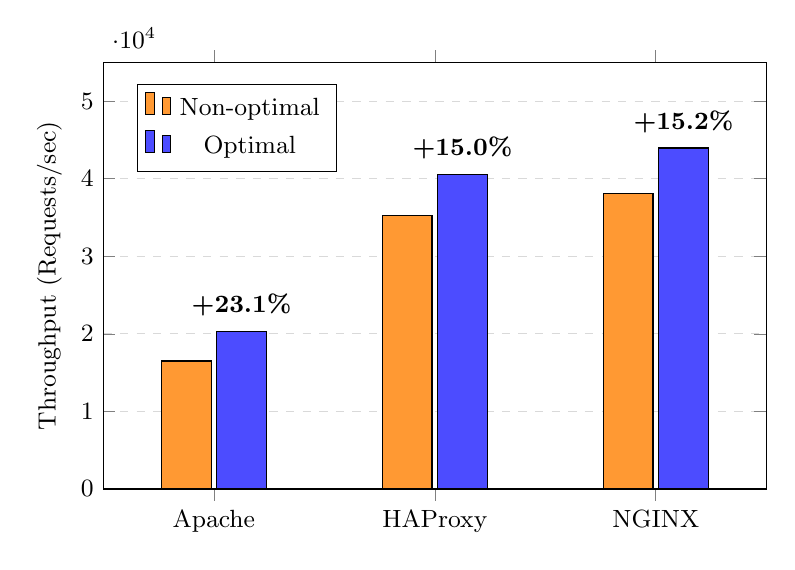
\begin{tikzpicture}
        \begin{axis}[
            ybar=2pt, % Space between the bars in a group
            bar width=18pt,
            width=10cm,
            height=7cm,
            enlarge x limits=0.25,
            ymin=0, ymax=55000, 
            ylabel={Throughput (Requests/sec)},
            symbolic x coords={Apache, HAProxy, NGINX},
            xtick=data,
            ymajorgrids=true,
            grid style={dashed, gray!30},
            axis line style={black},
            tick label style={font=\small},
            label style={font=\small},
            legend style={
                at={(0.05,0.95)}, 
                anchor=north west, 
                nodes={inner sep=3pt, font=\small},
                draw=black
            },
            % CHANGED: 'bottom' to 'south'
            every node near coord/.append style={
                font=\bfseries\small,
                anchor=south, 
                yshift=2pt
            }
        ]
        
        % --- Worst Avg (First Bar) ---
        \addplot[fill=orange!80!white, draw=black] coordinates {
            (Apache, 16498.62) 
            (HAProxy, 35262.75) 
            (NGINX, 38139.37)
        };
        
        % --- Top Avg (Second Bar) with Explicit Percentage Labels ---
        \addplot[
            fill=blue!70!white, 
            draw=black,
            nodes near coords,
            point meta=explicit symbolic 
        ] coordinates {
            (Apache, 20313.20) [+23.1\%]
            (HAProxy, 40550.52) [+15.0\%]
            (NGINX, 43953.42) [+15.2\%]
        };
        
        \legend{Non-optimal, Optimal}
        
        \end{axis}
    \end{tikzpicture}
    \caption{Throughput improvements achieved via Bayesian Optimization. The chart compares the average throughput of the non-optimal and optimal \textit{sysctl} configurations evaluated during the search space exploration.}
    \label{fig:optimization_throughput}
\end{figure}

\subsection{Workload Characterization} \label{subsec:workload}

To accurately evaluate the impact of the critical \textit{sysctl} knobs identified by the static analysis, it is essential to subject the target applications to distinct traffic patterns.
Different network behaviours traverse different execution paths within the Linux kernel, thereby shifting the system bottlenecks.
To simulate these varying conditions, the HTTP benchmarking tool \texttt{wrk} (version 5.2.0) was utilized to generate two distinct load profiles.

Testing different workloads is a crucial aspect of this evaluation because a "one-size-fits-all" configuration does not exist within the Linux kernel.
A parameter that maximizes raw data throughput (such as vastly expanding TCP memory buffers) might inadvertently increase queuing delays (buffer-bloat), thus severely degrading latency.
In contrast, optimizing the kernel for rapid connection cycling can introduce CPU overhead that degrades sustained data transfer rates.
By varying the workload, we can observe how system bottlenecks dynamically shift and how the automated tuning framework adapts its parameter selection accordingly.

\begin{itemize}
    \item \textbf{Workload A (High Concurrency / Short-Lived Connections)}: This profile was generated by repeatedly requesting a small, $\sim 1kB$ static file. Because the payload is negligible, the network transaction completes almost instantly. This workload forces the server to constantly open and close thousands of connections per second. It aggressively stresses the kernel connection management subsystem, specifically testing the efficiency of TCP handshakes and teardowns, the capacity of the \texttt{SYN} backlog, and the management of sockets in the \texttt{TIME\_WAIT} state.
    \item \textbf{Workload B (High Throughput / Large Payloads)}: this profile was generated by requesting the default \textit{test.html} file provided by wrk, which is approximately $\sim 100kB$ in size. In this scenario, the server handles fewer overall connection requests but must push significantly more data per connection. This workload shifts the primary system bottleneck away from connection establishment and places it squarely on the kernel data transmission mechanisms. It heavily stresses TCP window scaling, socket memory buffer allocations, and congestion control algorithms to ensure high-bandwidth data delivery.
\end{itemize}

By evaluating the web servers against both the $\sim 1KB$ and $\sim 100KB$ payloads, the resulting data clearly shows how the criticality of specific \textit{sysctl} knobs fluctuates based on the application execution context.

\subsection{Architectural Impact on Tuning: NGINX vs. Apache}

Before analysing the specific parameters identified by the tuning framework, it is necessary to establish why different applications require fundamentally different kernel configurations.
The optimal state of the kernel networking stack is intrinsically related to the user-space architecture of the application that interacts with it.
To demonstrate this, we contrast two of the most widely deployed web servers: NGINX and Apache HTTP Server.

\subsubsection{NGINX Architecture}

NGINX utilizes an asynchronous, event-driven architecture built  on I/O multiplexing mechanisms like \texttt{epoll}.
Rather than spawning a new thread or process for every incoming request, NGINX relies on a small number of single-threaded worker processes.
Each worker operates a highly efficient event loop capable of managing thousands of concurrent connections simultaneously without blocking (left side Figure~\ref{fig:arch_comparison}).
Because the user-space overhead for connection management is exceptionally low, NGINX rarely suffers from thread exhaustion or severe context-switching penalties.
Consequently, the performance bottleneck for NGINX rarely lies in how the kernel schedules user-space threads.
Instead, it rapidly shifts to the raw data transmission capabilities of the kernel.
For NGINX to achieve maximum throughput, the kernel must be optimized to push bytes across the network as aggressively as possible, making it highly sensitive to the dynamics of the TCP protocol, window scaling mechanisms, and congestion control algorithms.

\subsubsection{Apache Architecture}

Conversely, the Apache HTTP Server traditionally employs a process-driven or thread-driven architecture, depending on the configured Multi-Processing Module (e.g., Worker or Event MPM).
In these models, each active connection typically ties up a dedicated OS thread or process (right side Figure~\ref{fig:arch_comparison}.
Although robust, this design implies that Apache consumes significantly more heavy user-space resources per connection than NGINX.
As concurrency scales, the operating system is forced to perform frequent context switches to manage the multitude of active threads.
As a result, Apache performance is highly sensitive to CPU contention and how the kernel handles network I/O notifications.
Kernel mechanisms designed to reduce micro-second network latency by aggressively consuming CPU cycles (such as actively polling network device queues instead of relying on hardware interrupts) can starve Apache worker threads of the CPU time they need to process requests.

\begin{figure}[htbp]
    \centering
    \resizebox{\textwidth}{!}{
        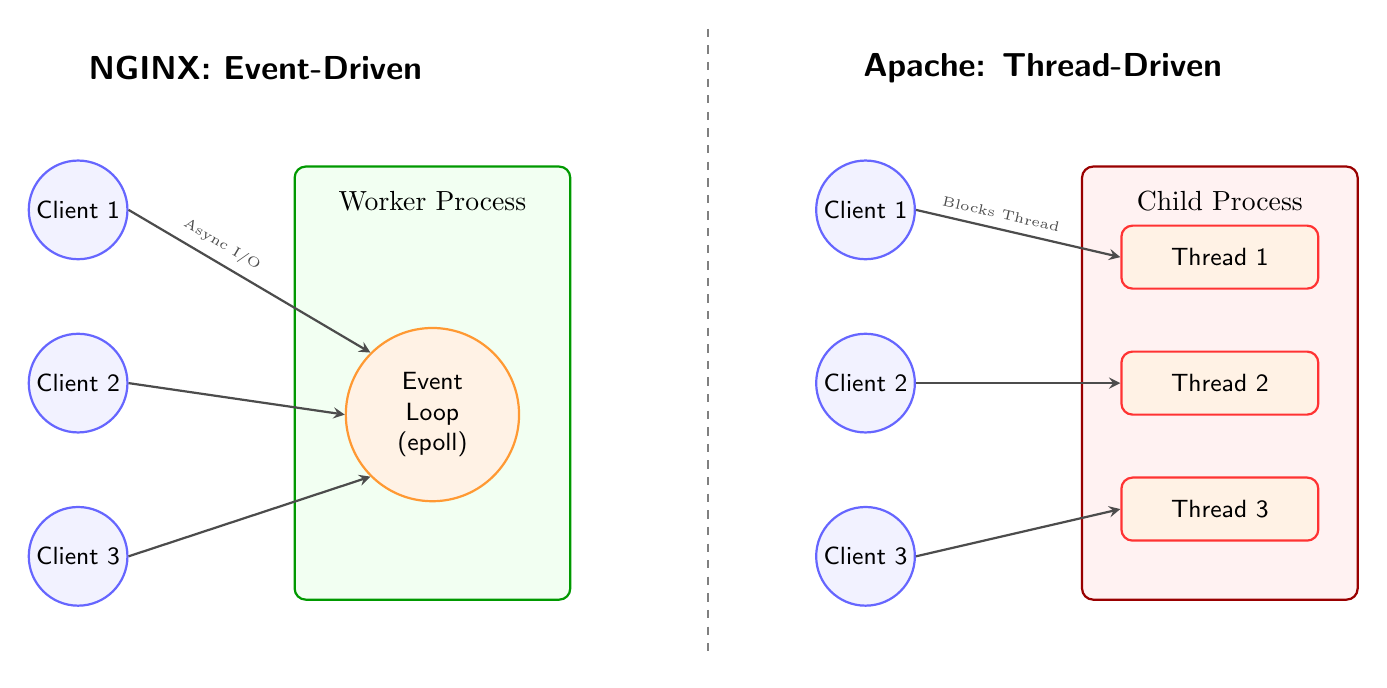
\begin{tikzpicture}[
            >=stealth, thick,
            client/.style={circle, draw=blue!60, fill=blue!5, minimum size=1.2cm, inner sep=2pt, font=\sffamily\small},
            worker/.style={rectangle, draw=green!60!black, fill=green!5, minimum width=3.5cm, minimum height=5.5cm, rounded corners, font=\sffamily\bfseries},
            eventloop/.style={circle, draw=orange!80, fill=orange!10, minimum size=2.2cm, align=center, font=\sffamily\small},
            apacheproc/.style={rectangle, draw=red!60!black, fill=red!5, minimum width=3.5cm, minimum height=5.5cm, rounded corners, font=\sffamily\bfseries},
            thread/.style={rectangle, draw=red!80, fill=orange!10, minimum width=2.5cm, minimum height=0.8cm, rounded corners, font=\sffamily\small},
            title/.style={font=\sffamily\large\bfseries}
        ]

        % ==========================================
        % LEFT SIDE: NGINX (Event-Driven)
        % ==========================================
        \node[title] (nginxtitle) at (0.75, 4) {NGINX: Event-Driven};
        
        % Clients (Increased vertical spacing to prevent touching)
        \node[client] (nc1) at (-1.5, 2.2) {Client 1};
        \node[client] (nc2) at (-1.5, 0) {Client 2};
        \node[client] (nc3) at (-1.5, -2.2) {Client 3};

        % Worker Process & Event Loop
        \node[worker] (nworker) at (3, 0) {};
        \node[anchor=north, yshift=-0.2cm] at (nworker.north) {Worker Process};
        \node[eventloop] (nloop) at (3, -0.4) {Event\\Loop\\(epoll)};

        % Connections
        \draw[->, color=black!70] (nc1.east) -- (nloop.135) node[midway, above, sloped, font=\tiny, pos=0.35] {Async I/O};
        \draw[->, color=black!70] (nc2.east) -- (nloop.180);
        \draw[->, color=black!70] (nc3.east) -- (nloop.225);

        % ==========================================
        % RIGHT SIDE: APACHE (Thread-Driven)
        % ==========================================
        % Shifted right to 10cm to give more breathing room for the center line
        \begin{scope}[xshift=10cm]
            \node[title] (apachetitle) at (0.75, 4) {Apache: Thread-Driven};
            
            % Clients
            \node[client] (ac1) at (-1.5, 2.2) {Client 1};
            \node[client] (ac2) at (-1.5, 0) {Client 2};
            \node[client] (ac3) at (-1.5, -2.2) {Client 3};

            % Child Process & Threads
            \node[apacheproc] (aworker) at (3, 0) {};
            \node[anchor=north, yshift=-0.2cm] at (aworker.north) {Child Process};
            
            \node[thread] (at1) at (3, 1.6) {Thread 1};
            \node[thread] (at2) at (3, 0) {Thread 2};
            \node[thread] (at3) at (3, -1.6) {Thread 3};

            % Connections
            \draw[->, color=black!70] (ac1.east) -- (at1.west) node[midway, above, sloped, font=\tiny, pos=0.4] {Blocks Thread};
            \draw[->, color=black!70] (ac2.east) -- (at2.west);
            \draw[->, color=black!70] (ac3.east) -- (at3.west);
        \end{scope}

        % ==========================================
        % SEPARATOR
        % ==========================================
        % The left worker ends at x=4.75. The right clients start around x=8. 
        % Placing the dashed line exactly in the middle at x=6.5.
        \draw[dashed, color=gray] (6.5, 4.5) -- (6.5, -3.5);

        \end{tikzpicture}
    }
    \caption{Architectural comparison between NGINX asynchronous event-driven model and Apache traditional thread-per-connection model. This fundamental difference dictates which kernel \texttt{sysctl} parameters become critical performance bottlenecks.}
    \label{fig:arch_comparison}
\end{figure}

\subsubsection{Tuning Hypothesis}

Based on these structural differences, a clear divergence in the critical \textit{sysctl} knobs identified for each application is expected.
Because Apache ties connections to heavier user-space resources and relies heavily on thread scheduling, kernel parameters that dictate I/O polling behaviour, CPU cycle allocation, and rapid connection termination will be strictly critical to its throughput.

On the other hand, because NGINX handles connections with minimal user-space overhead, it will easily saturate the network interface.
Therefore, the NGINX critical execution path will be bounded primarily by the kernel-level TCP protocol rules—specifically, the mathematical algorithms governing how the kernel scales transmission windows and manages network congestion.

The subsequent application-specific analyses empirically validate this architectural difference.

\subsection{Application Analysis: NGINX}

The evaluation of NGINX focused on its asynchronous and event-driven capabilities when subjected to the default $\sim 100kB$ payload workload (\textit{workload B}~\ref{subsec:workload}).
Under this profile, the automated tuning framework successfully navigated the kernel parameter space to unlock significant performance improvements.

\paragraph{Performance Gains.}
The application of the Bayesian-optimized \textit{sysctl} configuration, as shown in Figure~\ref{fig:optimization_throughput} resulted in a throughput improvement of approximately 15\% over the non-optimal case.
As observed in the tuning profile scatter plots in Figure~\ref{fig:nginx_profiler}, the non-optimal configurations frequently stalled near 38,000 requests per second, while the optimal parameter combination reliably pushed throughput to a peak of over 43,500 requests per second.

\begin{figure}[htbp]
    \centering
    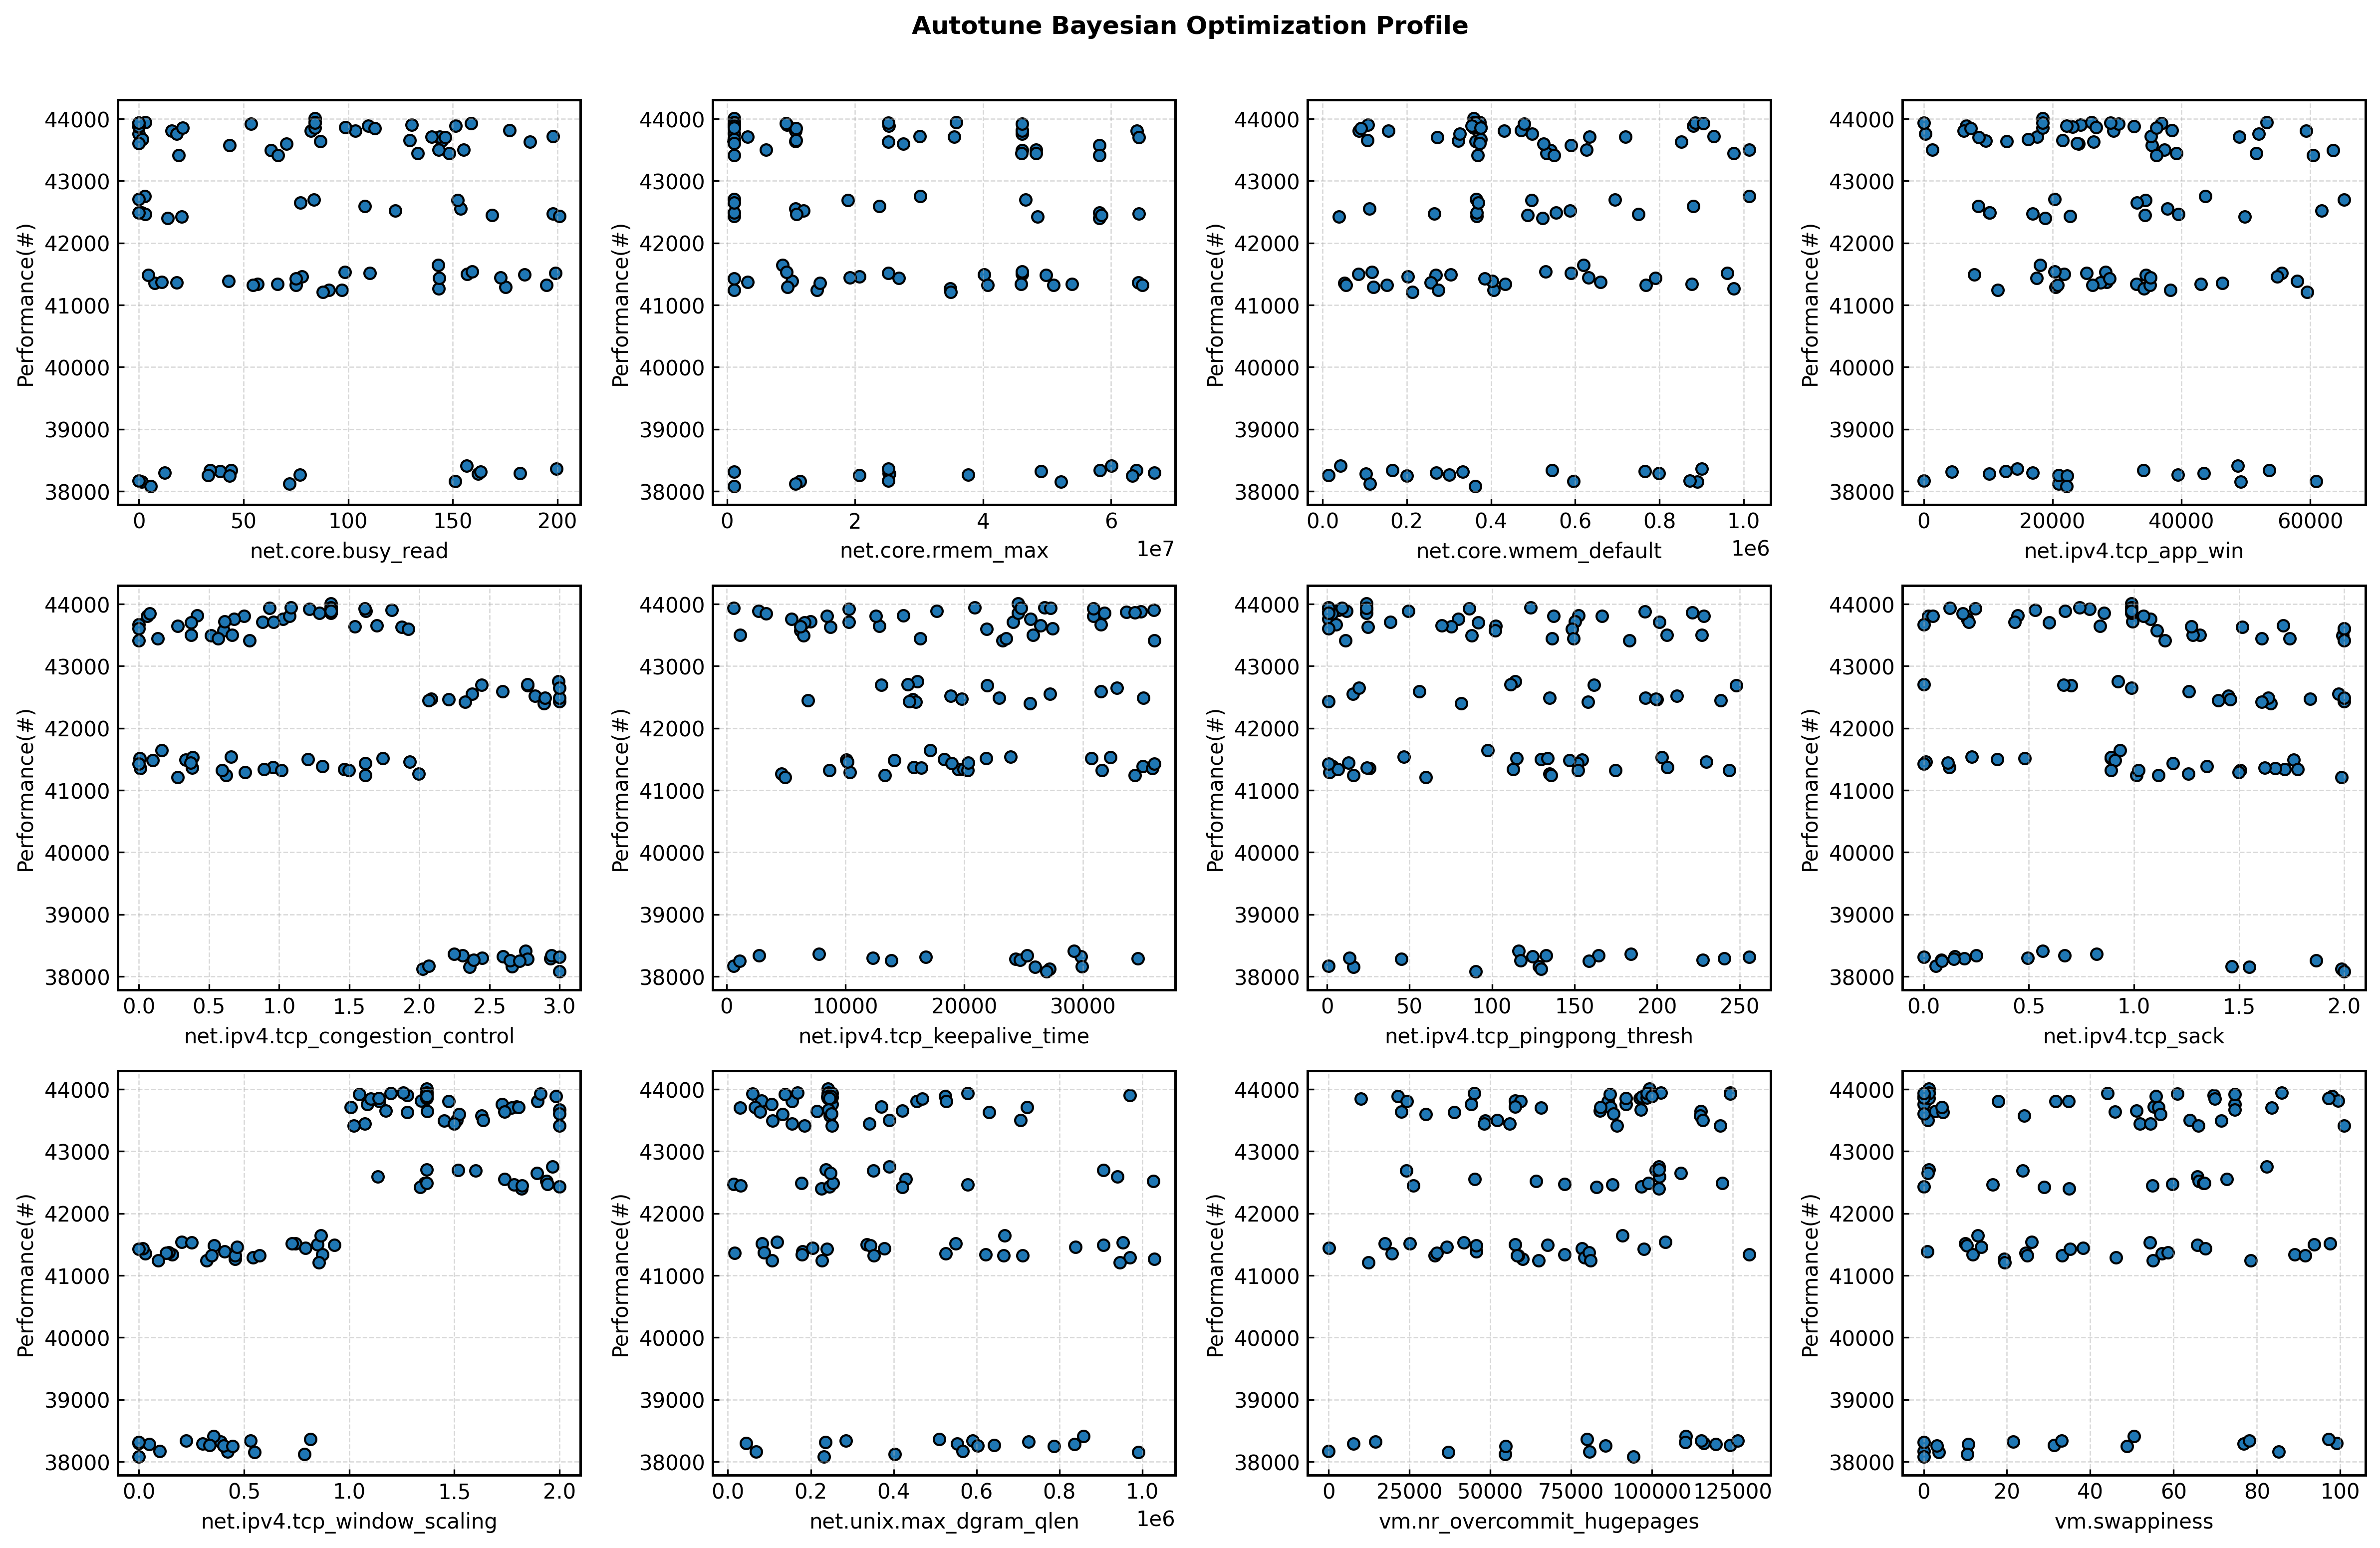
\includegraphics[width=0.95\linewidth]{images/5_evaluation/nginx/profiler.png}
    \caption{Performance profile for NGINX under the 100KB payload workload. Each subplot illustrates the relationship between the explored values of a specific \textit{sysctl} parameter (x-axis) and the resulting application throughput in requests per second (y-axis). For visual clarity, these subplots represent a filtered subset of the knobs from the full tuning space. The clustering of points at the upper and lower throughput boundaries illustrates how specific parameter values dictate overall system bottlenecks.}
    \label{fig:nginx_profiler}
\end{figure}

\paragraph{Critical Knobs Identified.}
By analysing the Partial Dependence Plot (PDP) generated by a Random Forest~\cite{random_forests} surrogate model in Figure~\ref{fig:nginx_pdp}, we can isolate the specific kernel parameters that most heavily influenced this performance delta.
For NGINX with 100KB workload, the three most critical knobs were \texttt{net.ipv4.tcp\_window\_scaling}, \texttt{net.ipv4.tcp\_congestion\_control}, and \texttt{net.ipv4.tcp\_sack}.

\begin{figure}[htbp]
    \centering
    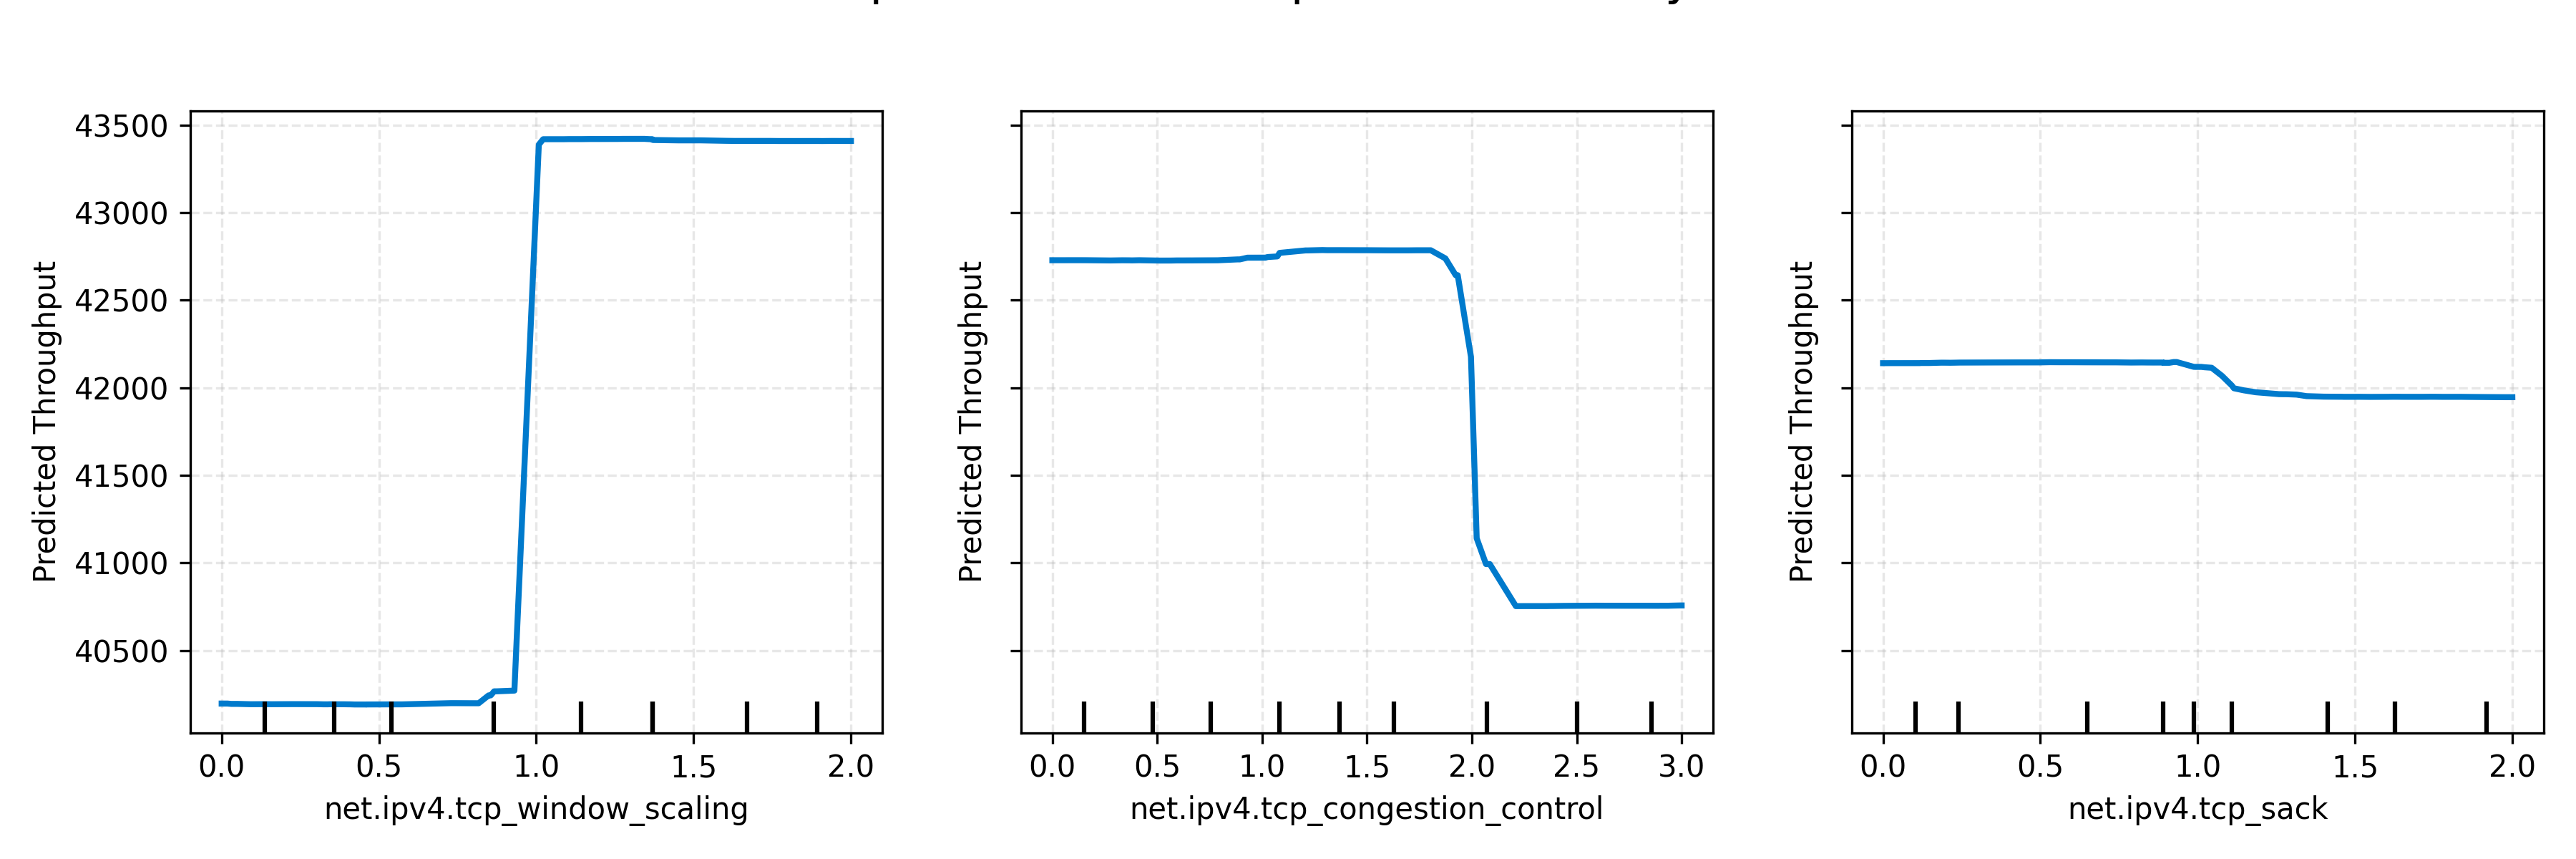
\includegraphics[width=0.8\linewidth]{images/5_evaluation/nginx/pdp.png}
    \caption{Partial Dependence Plots (PDP) isolating the marginal effect of the three most influential \textit{sysctl} knobs on NGINX throughput. The sharp step-function in the leftmost plot demonstrates a critical performance threshold, indicating that throughput drastically increases once \texttt{tcp\_window\_scaling} is enabled ($\ge 1.0$). The center plot illustrates performance degradation associated with higher indices of \texttt{tcp\_congestion\_control}.}
    \label{fig:nginx_pdp}
\end{figure}

\paragraph{Architectural Justification.}
The identification of these specific parameters perfectly aligns with NGINX architectural design.
Because the \textit{epoll}-based worker processes handle connection establishment with extreme efficiency, the performance bottleneck immediately shifts to the kernel raw data transmission mechanics.

The 100 KB payload size is particularly revealing because it exceeds the fundamental limits of the original TCP specification.
The standard TCP header allocates only 16 bits for the receive window, capping the maximum unscaled window size at exactly roughly 64 KB~\cite{tcp_window_scale}.
The Partial Dependence Plot (PDP) shown in Figure~\ref{fig:nginx_pdp} illustrates a massive, step-function increase in throughput exactly at the threshold where \texttt{tcp\_window\_scaling} is enabled (values $\ge 1.0$).
This parameter activates RFC 7323, allowing the kernel to mathematically shift the window size to support massively larger buffers.

Without window scaling, the kernel can only transmit 64 KB of the 100 KB payload before it is strictly forced to halt transmission and wait for client acknowledgments.
This mandatory pause introduces network latency that effectively starves NGINX rapid event loop.
Once scaling is enabled, the advertised window safely exceeds the 100 KB threshold, allowing the kernel to push the entire payload to the socket buffer and transmit it continuously without mid-stream acknowledgment stalls~\cite{tcp_window_scale}.

Furthermore, the data shows that throughput decreases significantly when the \texttt{tcp\_congestion\_control} parameter index exceeds 2.0.
This parameter dictates the algorithmic strategy the kernel uses to infer network capacity and regulate its transmission rate.
The results indicate that traditional, loss-based algorithms (such as Reno or CUBIC, which map to the lower indices) are vastly superior for this specific workload compared to BBR, which is located at a higher index in the tested grid ($\ge 2.0$.

Loss-based algorithms aggressively and exponentially expand their congestion window until a packet is explicitly dropped.
In a controlled, high-bandwidth virtualized benchmarking environment, packet loss is virtually non-existent, allowing CUBIC and Reno to rapidly ramp up and completely saturate the link.
On the other hand, BBR is a delay-based algorithm that intentionally paces its sending rate to match the estimated bottleneck bandwidth, actively trying to prevent buffer queues.
For short 100 KB burst transfers in a local network, BBR mandatory bandwidth-probing phases and strict pacing introduce overhead that prevents it from achieving the unconstrained raw throughput of its loss-based counterparts.

\paragraph{Parameter Interaction.}
The Bayesian optimizer also revealed critical dependencies between these parameters.
The 2D interaction heat-map, shown in Figure~\ref{fig:nginx_2d_heatmap}, explicitly demonstrates that peak throughput (the bright yellow region) is exclusively achieved when \texttt{tcp\_window\_scaling} is enabled in parallel with a \texttt{tcp\_congestion\_control} index below 2.0.
Optimizing one without the other results in sub-optimal network performance.

\begin{figure}[htbp]
    \centering
    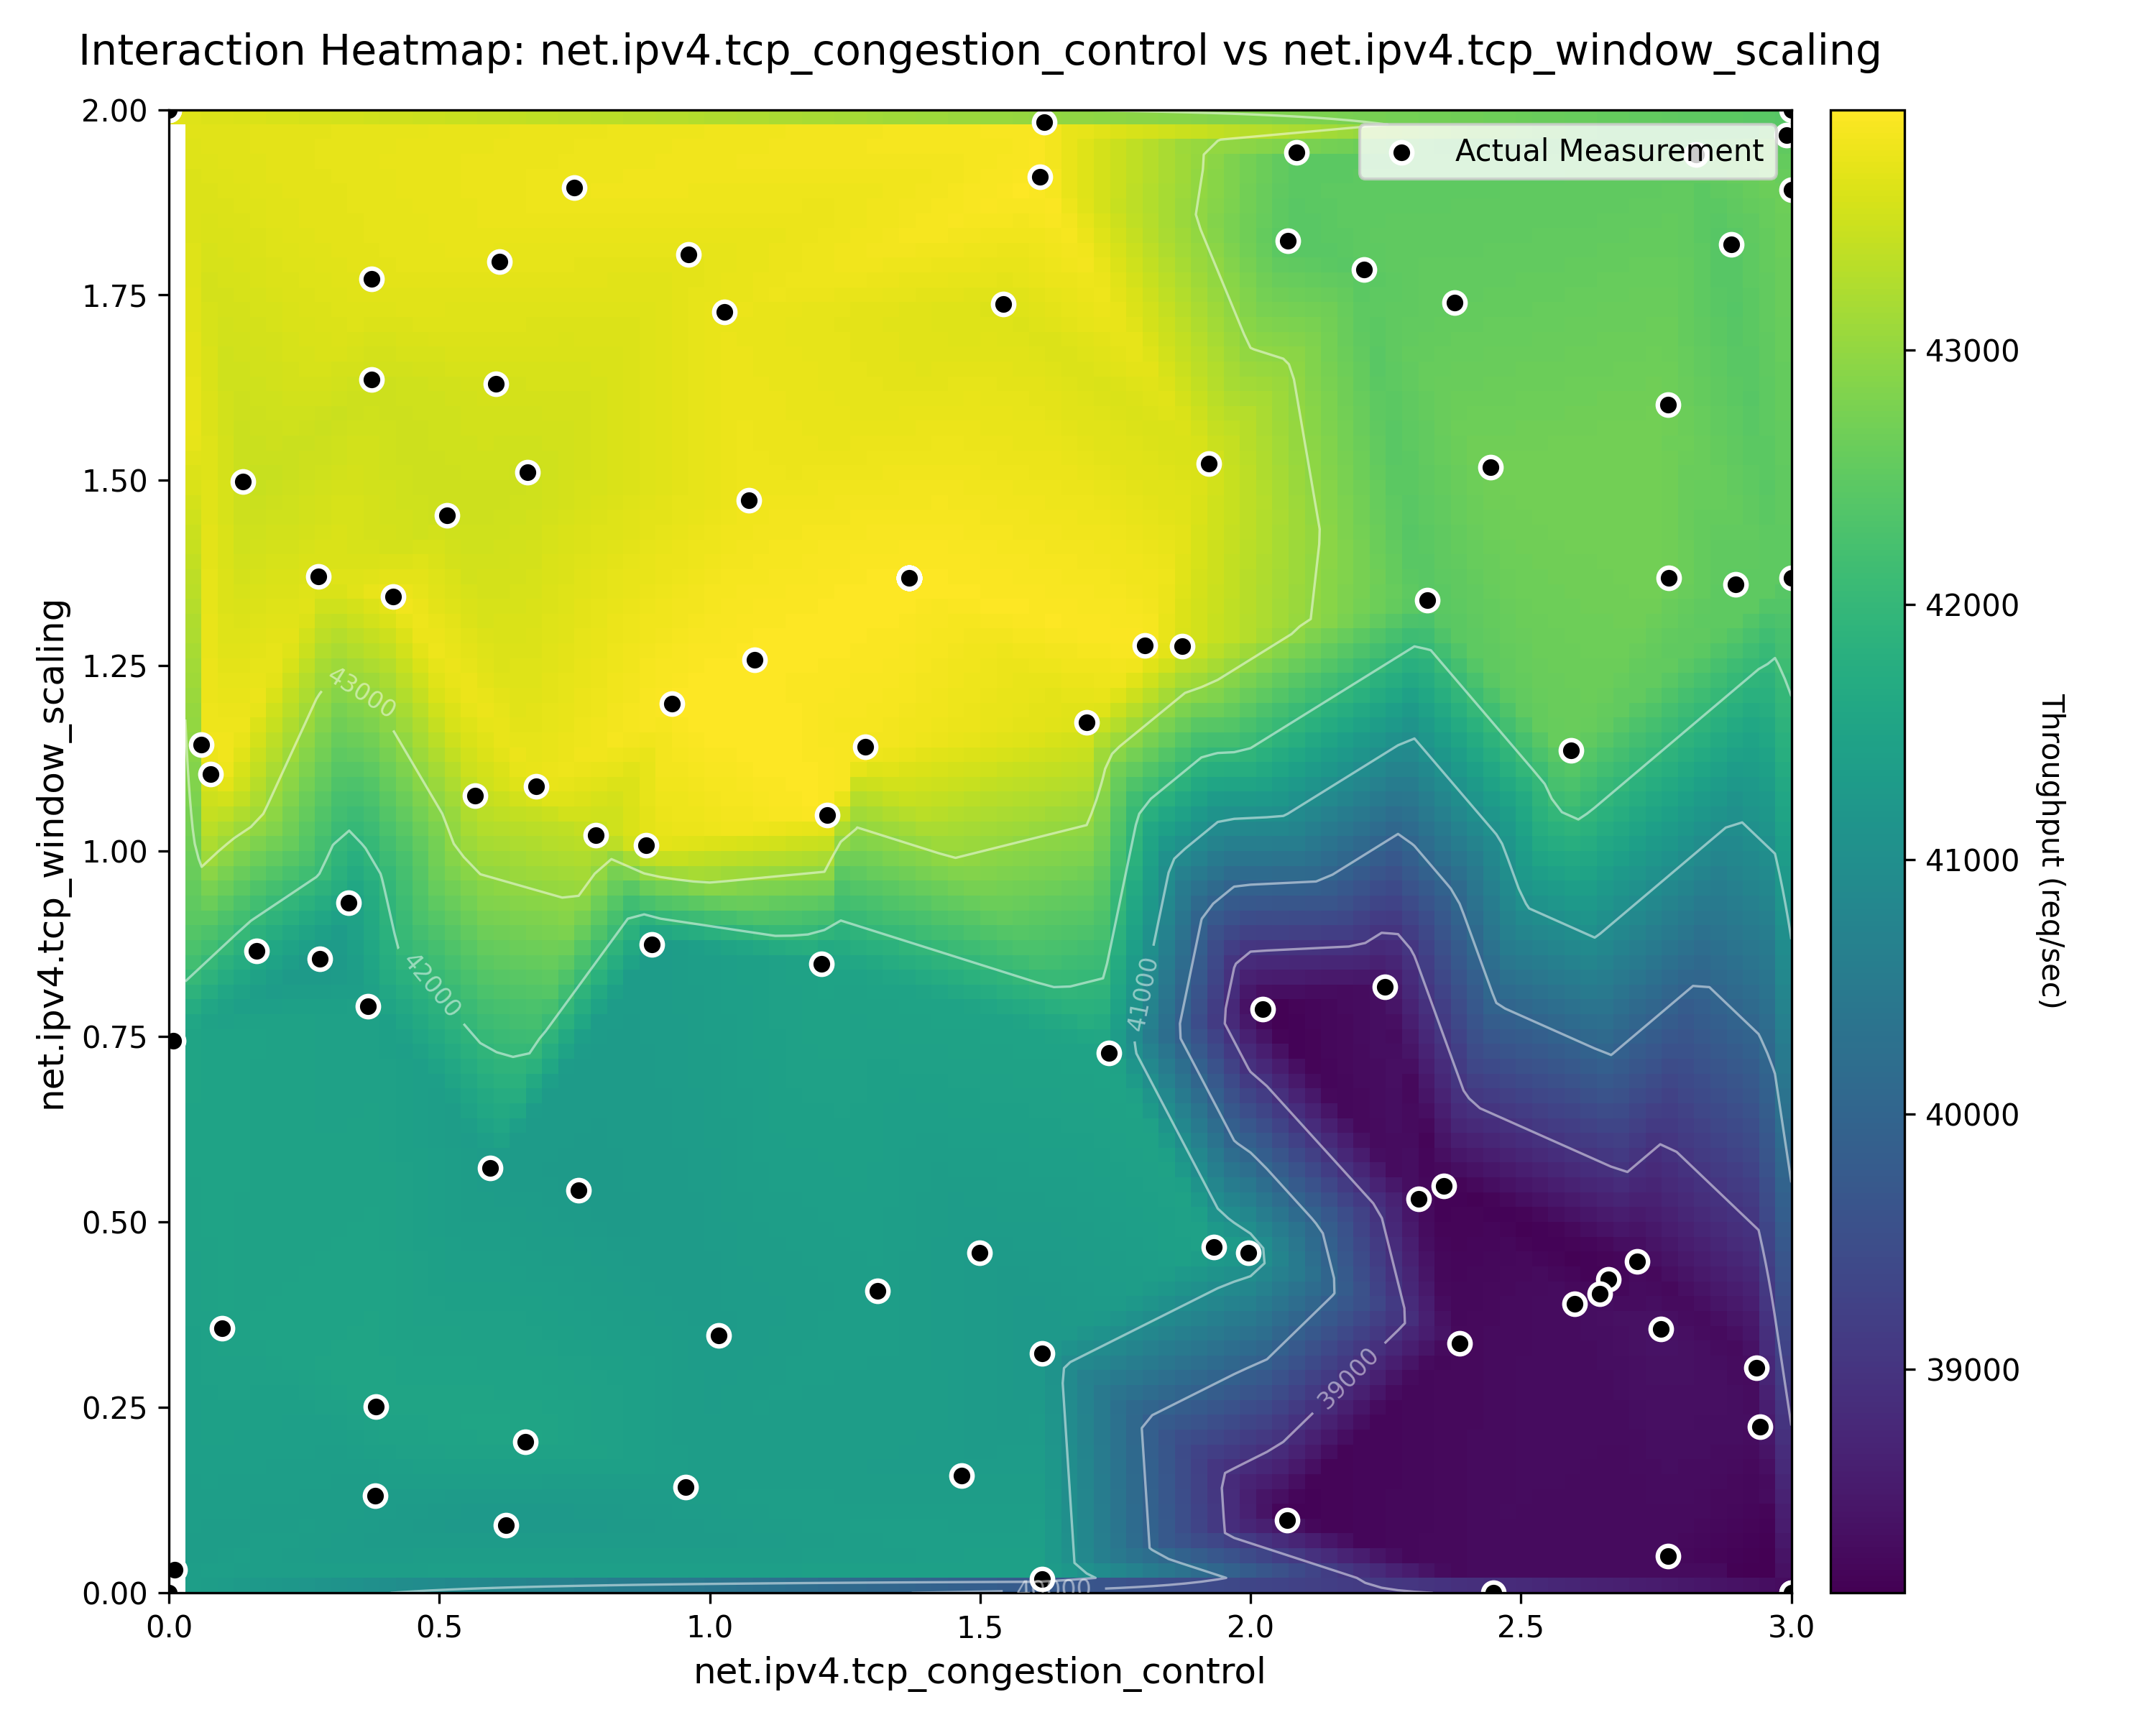
\includegraphics[width=0.65\linewidth]{images/5_evaluation/nginx/2d_heatmap.png}
    \caption{Two-dimensional interaction heat-map visualizing the combined effect of \texttt{tcp\_congestion\_control} (x-axis) and \texttt{tcp\_window\_scaling} (y-axis) on NGINX throughput. The bright yellow region indicates peak performance, confirming that maximum throughput is strictly achieved when window scaling is enabled in parallel with lower congestion control indices. Black dots represent actual measured configurations during the tuning phase.}
    \label{fig:nginx_2d_heatmap}
\end{figure}

Finally, an analysis of the top 10\% of all evaluated configurations confirms the optimizer certainty with respect to these bottlenecks.
The configuration heat-map (Figure~\ref{fig:nginx_heatmap}) shows that across all the best runs, the optimizer consistently locked \texttt{tcp\_window\_scaling} with values $\ge 1.0$ meaning that the window scaling is activated.

\begin{figure}[htbp]
    \centering
    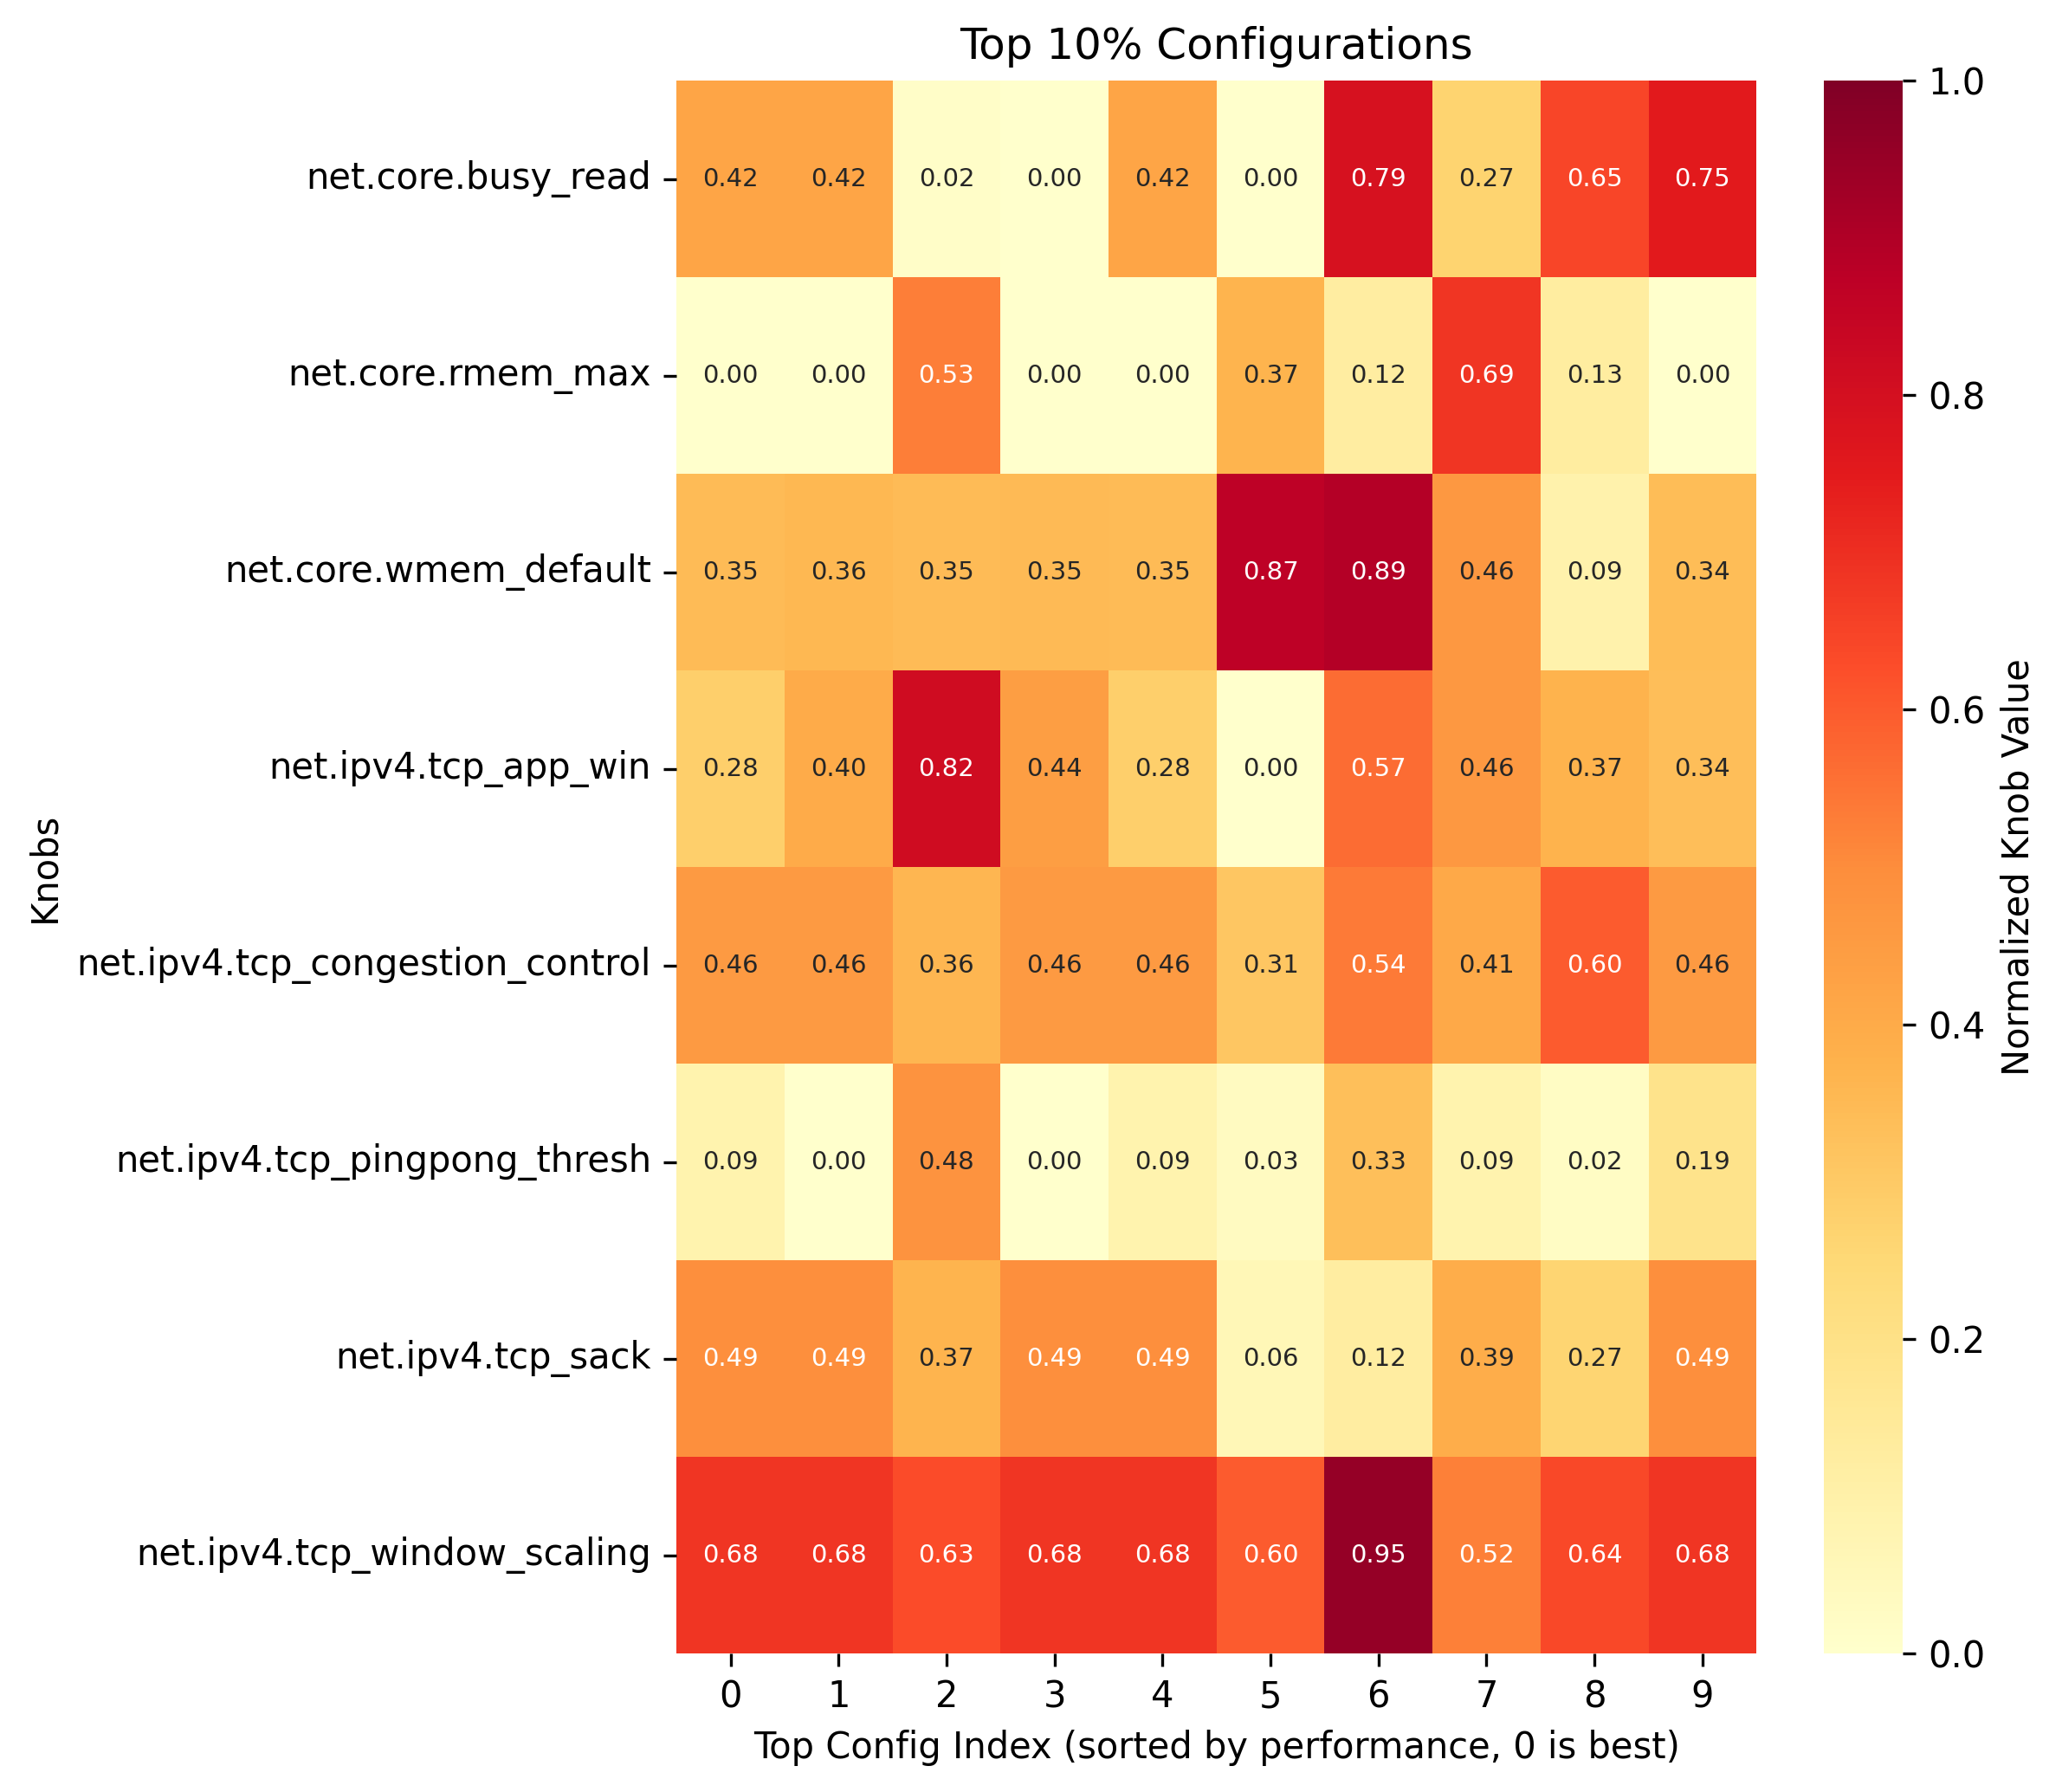
\includegraphics[width=0.65\linewidth]{images/5_evaluation/nginx/heatmap.png}
    \caption{Configuration heat-map displaying the normalized parameter values across the top 10\% highest-performing experimental runs for NGINX (where index 0 represents the absolute best configuration). For visual clarity, this figure displays only a subset of the most influential \texttt{sysctl} knobs from the full tuned set. Darker red shades indicate parameter values pushed toward their maximum explored limits, highlighting consistent optimizer behavior for critical knobs such as \texttt{tcp\_window\_scaling} and \texttt{tcp\_congestion\_control}.}
    \label{fig:nginx_heatmap}
\end{figure}

\subsection{Application Analysis: HAProxy}

Following the evaluation of NGINX, the automated tuning framework was applied to HAProxy under the identical $\sim 100KB$ payload workload.
Interestingly, the optimization results and the final set of critical parameters identified for HAProxy were almost completely identical to those of NGINX.
This parallel outcome provides strong empirical validation that an application underlying architectural paradigm, rather than its specific binary implementation, dictates its critical execution path through the kernel.

\paragraph{Performance Gains.}
Just like NGINX, HAProxy relies on an asynchronous, heavily optimized event loop (via \texttt{epoll}) to handle massive concurrency without dedicating heavily weighted threads to individual connections.
The Bayesian-optimized \textit{sysctl} configuration successfully capitalized on this architecture, yielding a throughput improvement of approximately 15\% (as shown in Figure~\ref{fig:optimization_throughput}).
The non-optimal configurations frequently plateaued near 35,500 requests per second, whereas the autotuned configurations consistently broke the 40,000 RPS threshold, peaking near 40,500 RPS.

\begin{figure}[htbp]
    \centering
    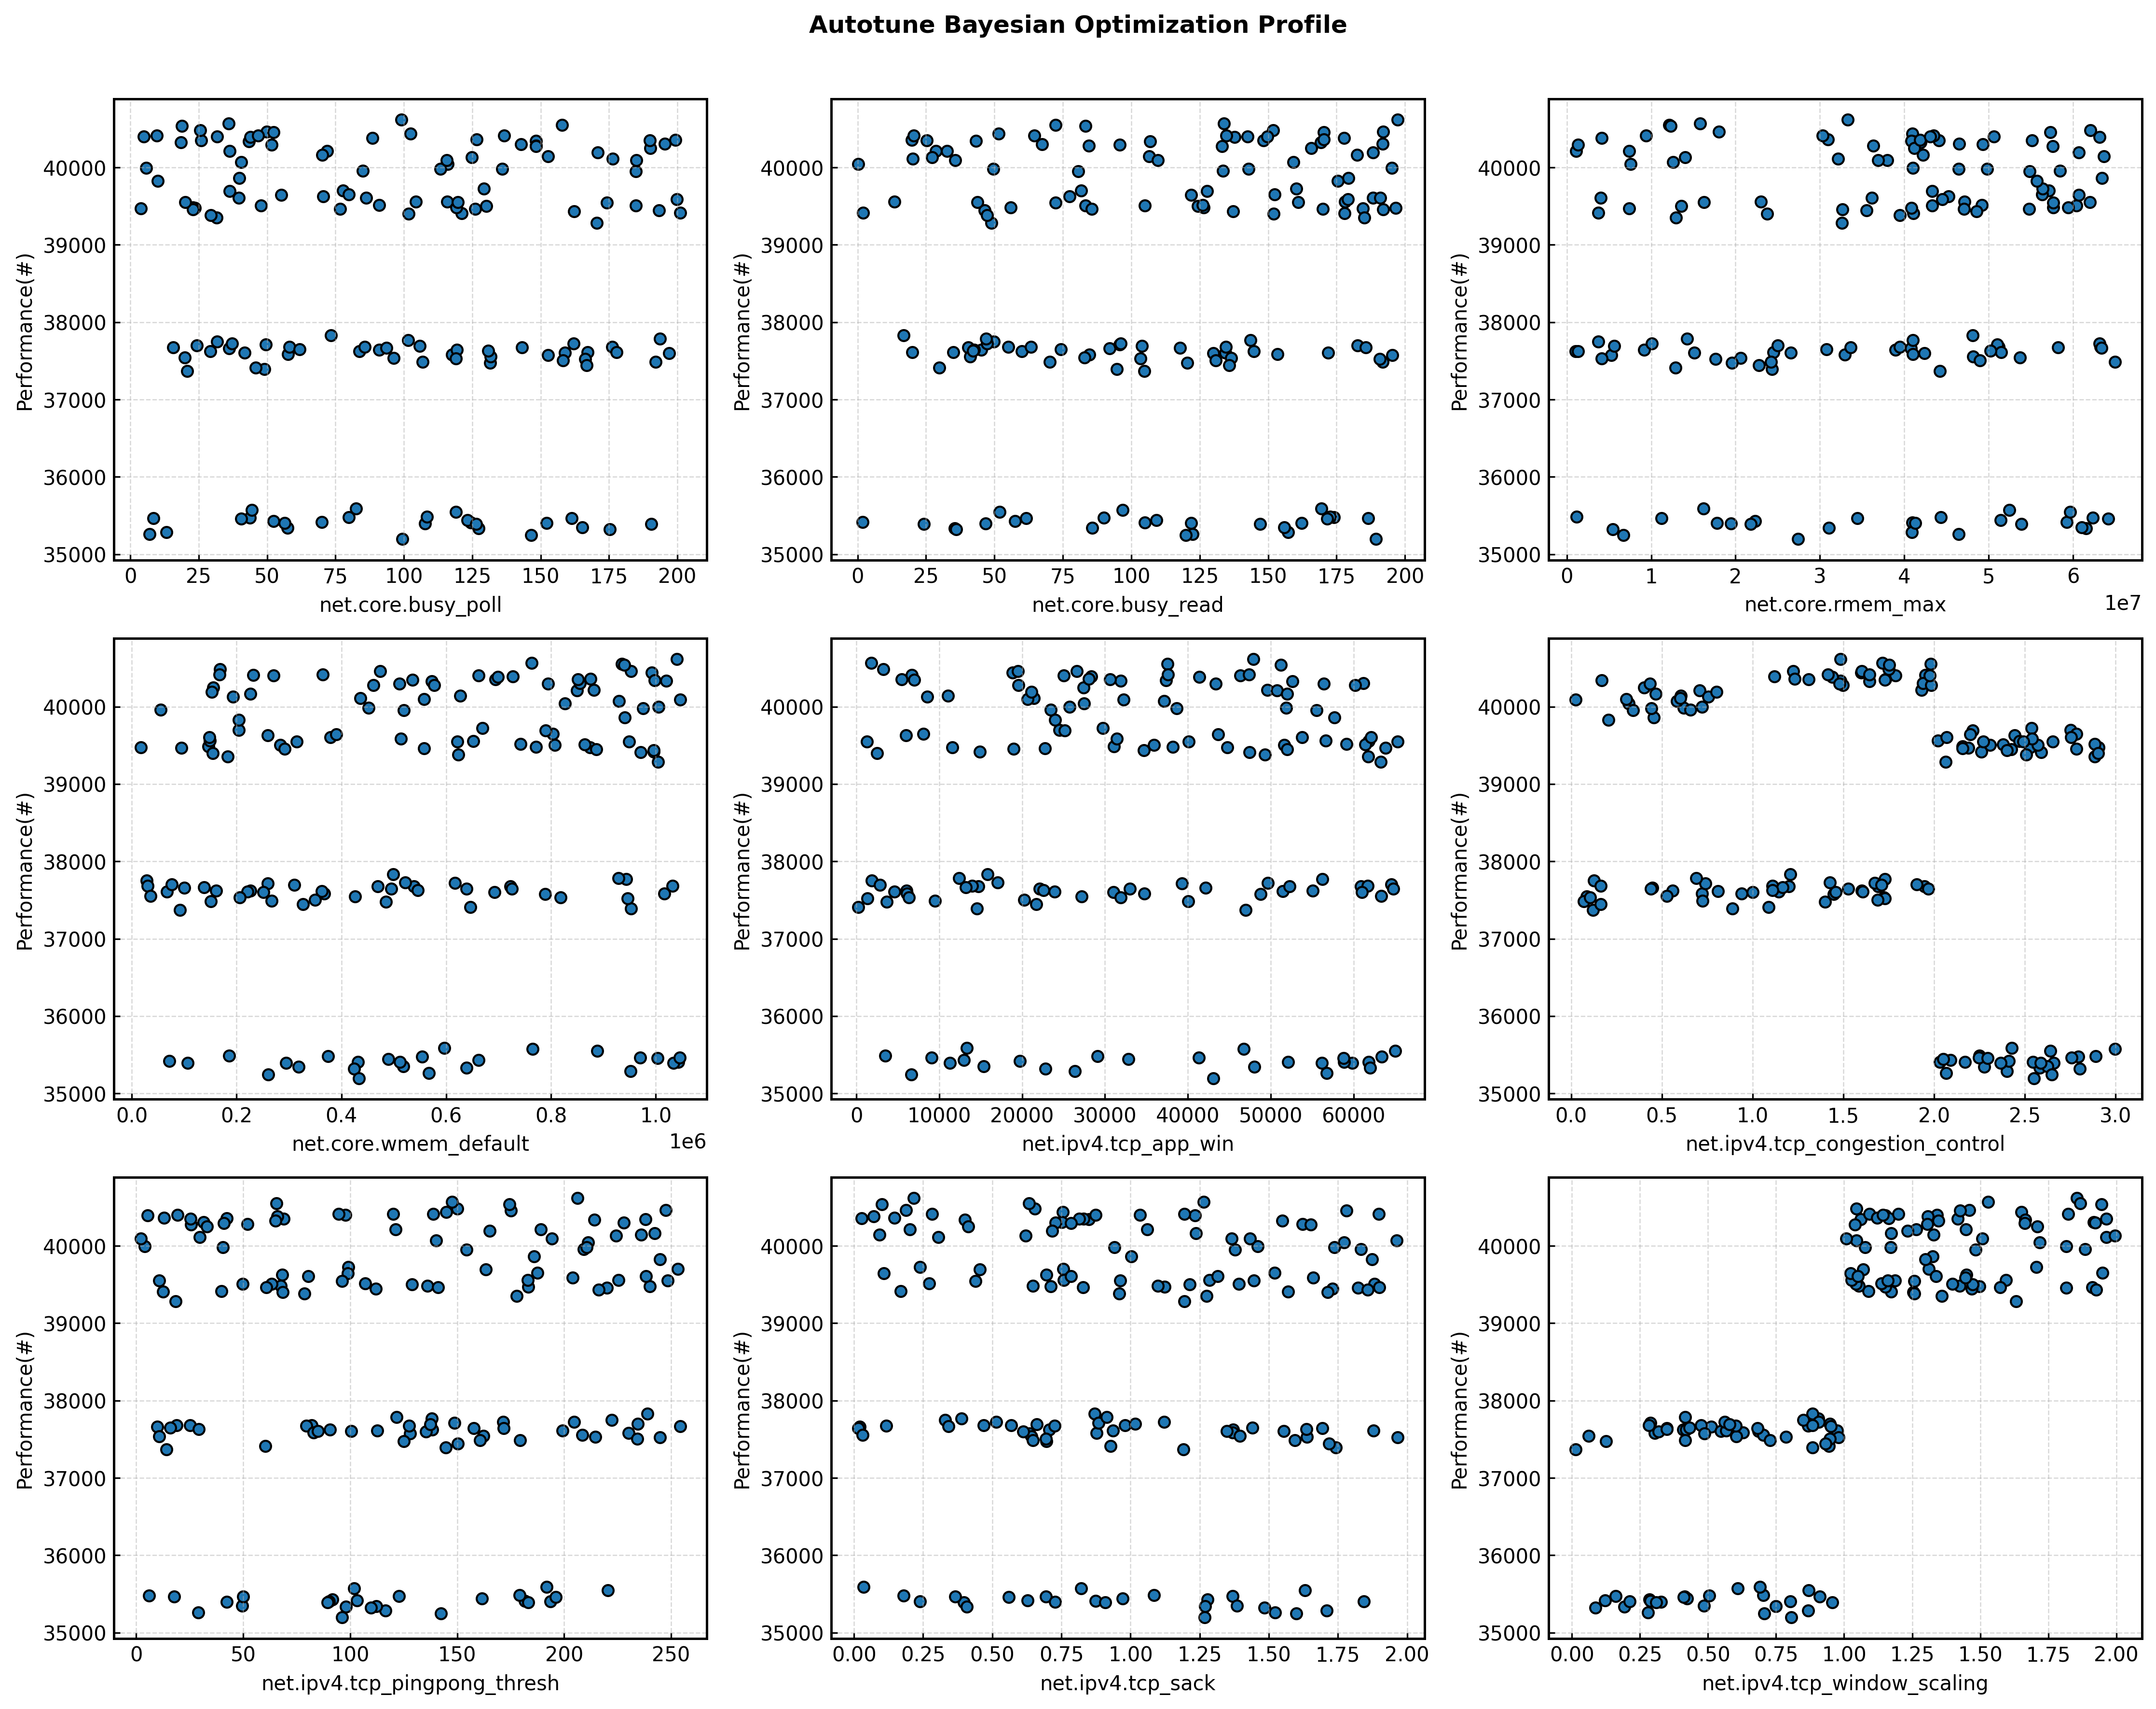
\includegraphics[width=0.85\linewidth]{images/5_evaluation/haproxy/profiler.png}
    \caption{Performance profile for HAProxy under the 100kB payload workload. Each subplot illustrates the relationship between the explored values of a specific \textit{sysctl} parameter (x-axis) and the resulting application throughput in requests per second (y-axis). For visual clarity, these subplots represent a filtered subset of the knobs from the full tuning space. The clustering of points at the upper and lower throughput boundaries illustrates how specific parameter values dictate overall system bottlenecks.}
    \label{fig:placeholder}
\end{figure}

\paragraph{Critical Knobs Identified and Architectural Justification.}
The Partial Dependence Plot (PDP) generated for HAProxy isolated the exact same primary bottlenecks as NGINX: \texttt{tcp\_window\_scaling} and \texttt{tcp\_congestion\_control}.

Because HAProxy acts as a highly efficient channel, reading data from a back-end and writing it to a client, it requires the kernel to push data as quickly as its event loop can multiplex it.
The 100KB payload again strictly exceeds the default 64KB TCP receive window.
Consequently, the PDP demonstrates a massive step-function increase in throughput exactly when \texttt{tcp\_window\_scaling} is enabled (values $\ge 1.0$).
Without this parameter, HAProxy is artificially throttled by the TCP protocol mandatory acknowledgment waits, stalling its rapid event loop.
Similarly, the throughput rapidly declines when the \texttt{tcp\_congestion\_control} parameter is set to \textit{BBR}.
This reaffirms that in a localized, low-packet-loss benchmarking environment, aggressive loss-based congestion algorithms (such as Reno or CUBIC) allow the proxy to fully saturate the network link much more effectively than delay-paced algorithms like \textit{BBR}.

\paragraph{Parameter Interaction.}
The interaction dynamics observed in HAProxy 2D heat-map and the top 10\% normalized configuration heat-map are almost identical to those of NGINX.
The region of peak throughput strictly correlates to the exact same relationship: \texttt{tcp\_window\_scaling} must be active alongside a \texttt{tcp\_congestion\_control} index below 2.0.
This remarkable similarity conclusively demonstrates that HAProxy and NGINX share the same critical execution path through the kernel.

\subsection{Application Analysis: Apache HTTP Server}

Following the evaluation of the event-driven architectures, the tuning framework was applied to the Apache HTTP Server.
Because Apache relies on a heavier, thread-based Multi-Processing Module (MPM) to handle concurrency, the hypothesis projected that its critical execution path would shift away from raw TCP window scaling and toward CPU and thread scheduling bottlenecks.
The empirical results definitively validate this projection.

\paragraph{Performance Gains.}
The Bayesian optimization process successfully converged on a configuration that yielded, as shown in Figure~\ref{fig:optimization_throughput}, a +23.1\% total gain in throughput over the non-optimal one.
As illustrated in the optimization plot in Figure~\ref{fig:apache_convergence}, the runs with a non-optimal configuration frequently drop around 16,500 requests per second, whereas the optimal configuration rapidly climbed, eventually plateauing at a peak performance around 20,500 RPS.

\begin{figure}[htbp]
    \centering
    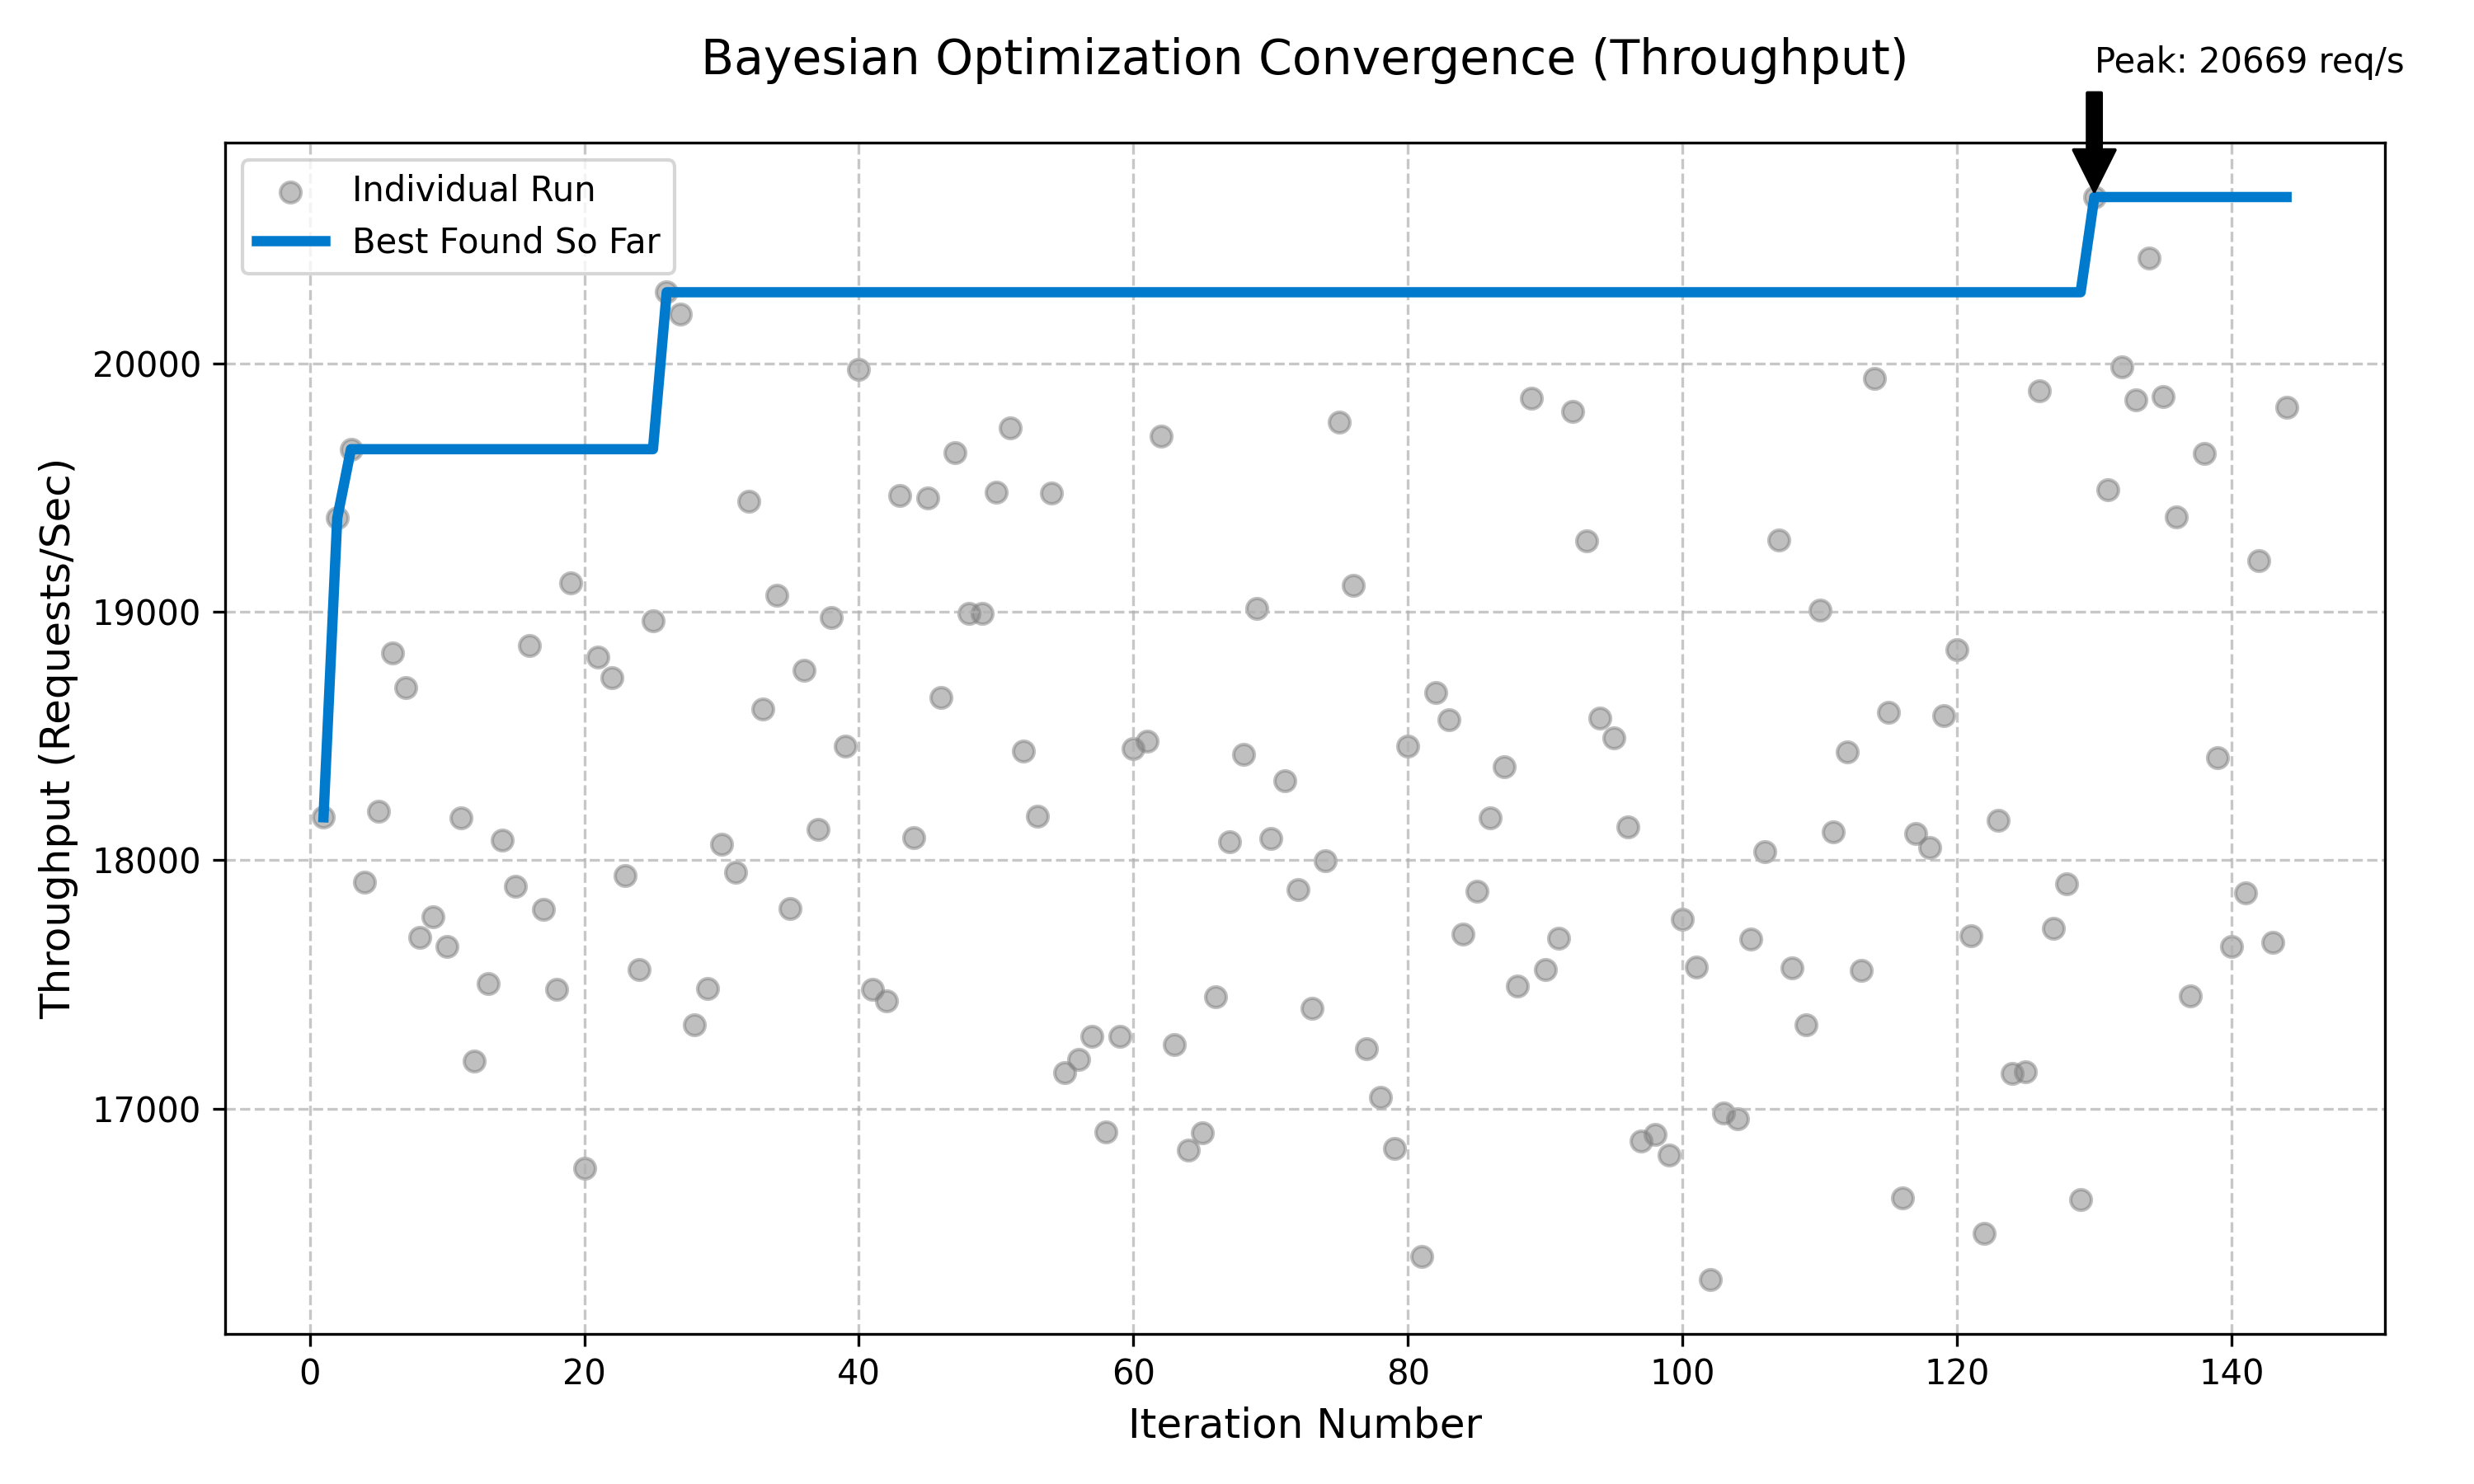
\includegraphics[width=0.7\linewidth]{images/5_evaluation/apache/convergence.png}
    \caption{Bayesian optimization convergence trajectory for the Apache HTTP Server. The graph tracks the throughput of individual experimental runs (dots) alongside the best configuration found so far (solid line). The optimization process successfully navigated the parameter space to achieve a peak throughput of 20,669 requests per second.}
    \label{fig:apache_convergence}
\end{figure}

\paragraph{Critical Knobs Identified.}
Unlike NGINX and HAProxy, where the Partial Dependence Plot highlighted the TCP scaling mechanisms, Apache PDP is overwhelmingly dominated by a single parameter: \texttt{net.core.busy\_poll}.
The surrogate model prediction curve (Figure~\ref{fig:apache_pdp}) for this parameter reveals a massive drop in predicted throughput as the value increases.

\begin{figure}[htbp]
    \centering
    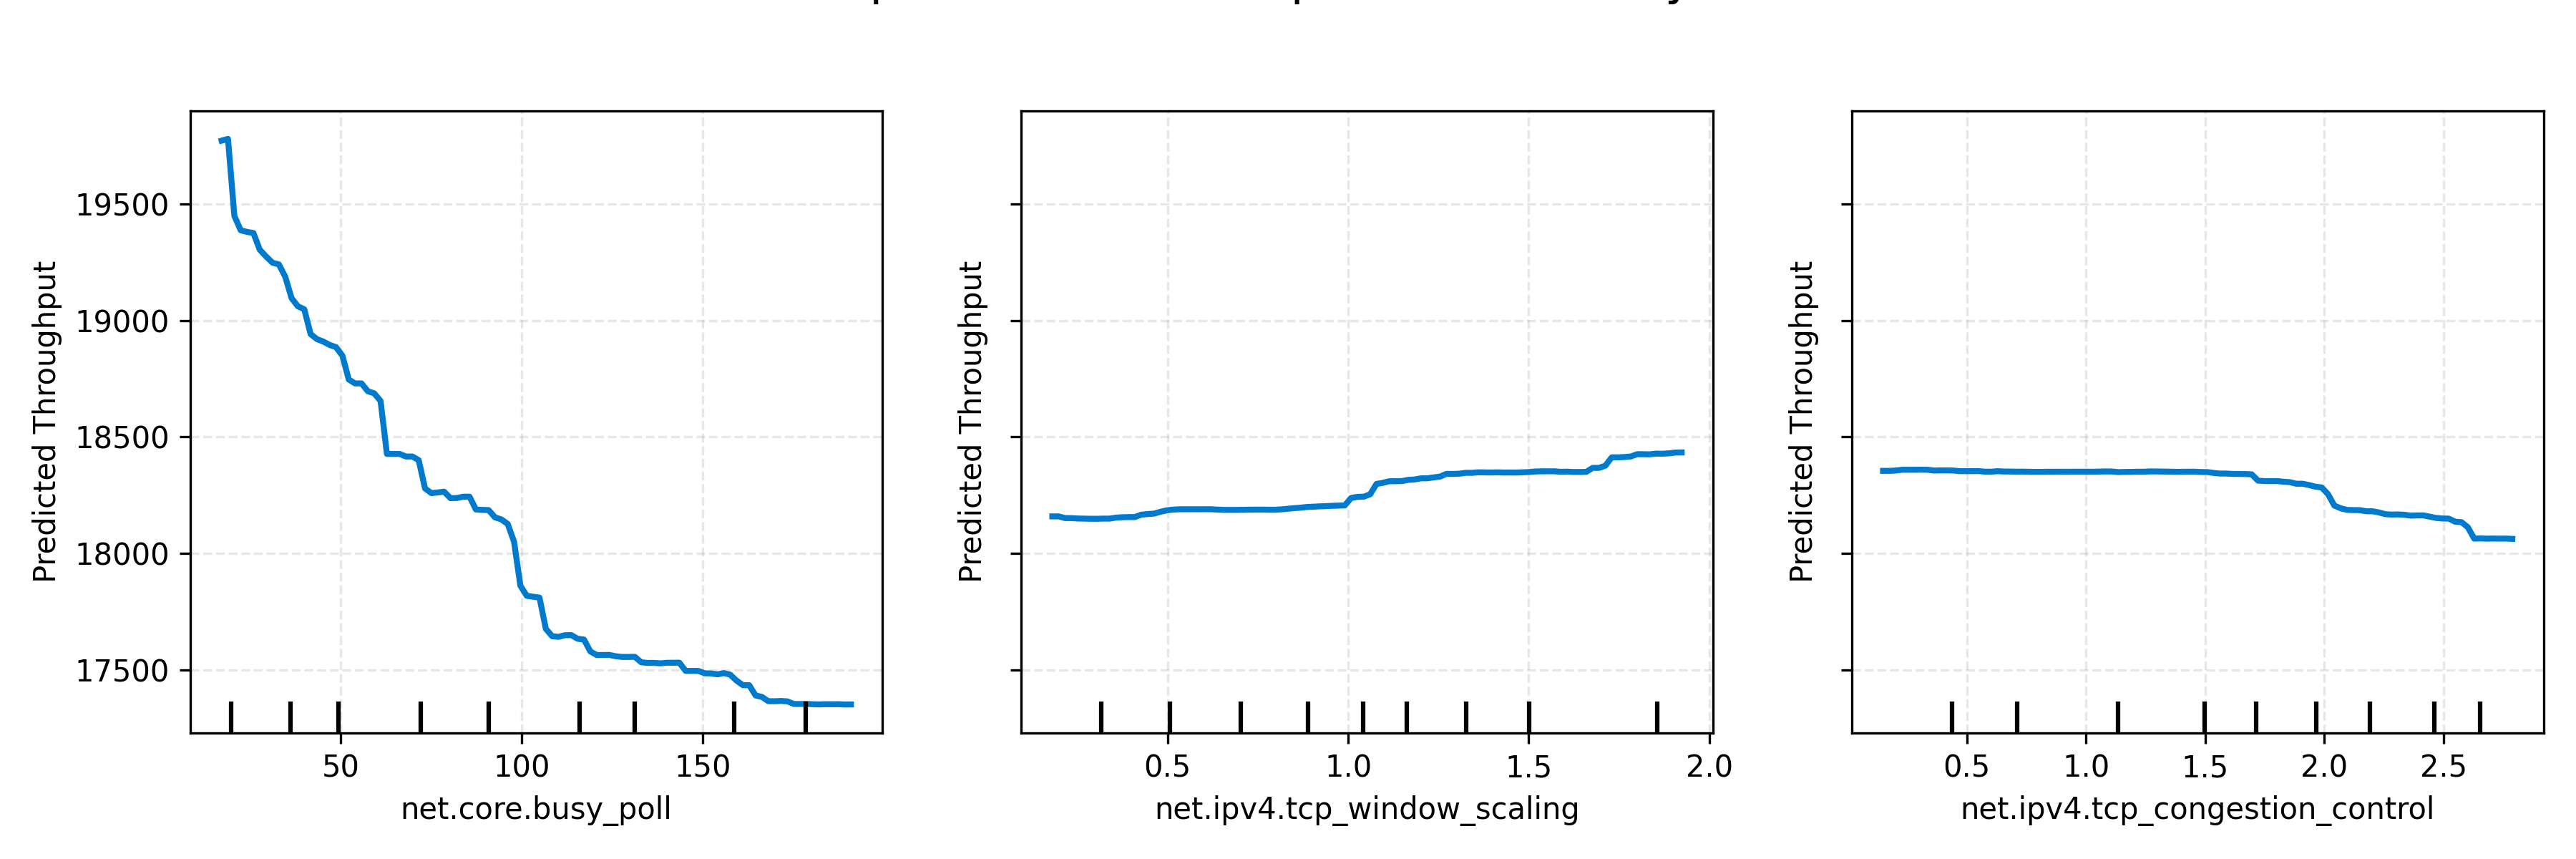
\includegraphics[width=0.8\linewidth]{images/5_evaluation/apache/pdp.png}
    \caption{Partial Dependence Plot (PDP) illustrating the isolated marginal effect of the most influential kernel parameters on Apache predicted throughput. The steep downward curve in the first subplot explicitly demonstrates how increasing the \texttt{busy\_poll} value severely penalizes the performance of thread-driven architectures by starving user-space processes of CPU cycles.}
    \label{fig:apache_pdp}
\end{figure}

\paragraph{Architectural Justification.}
The \texttt{busy\_poll} parameter controls the low-latency polling mechanism in the Linux network stack.
When set to a value greater than zero, it instructs the kernel to actively spin-wait (busy-poll) on the network device receive queues for incoming packets, rather than relying on hardware interrupts.
While busy-polling effectively reduces network latency by a few microseconds, it does so at a severe cost: it completely monopolizes CPU cycles in a tight spin loop.

For a highly asynchronous application like NGINX, occasionally burning CPU cycles on polling might not degrade overall throughput.
This is because NGINX utilizes a lean, event-driven architecture mapped directly to the available CPU cores, as demonstrated in Listing \ref{lst:nginx_pidstat}. However, for Apache thread-heavy architecture (Listing \ref{lst:apache_pidstat}), it results in a heavy performance degradation. 

Every CPU cycle spent actively polling the network card is a cycle stolen from Apache worker threads.
Because Apache requires these CPU cycles to context-switch, wake up dozens of concurrent threads, and process HTTP requests, the busy-polling mechanism directly starves the application of its most critical resource.
This is evidenced by the high \texttt{\%wait} times seen in the Apache process footprint.
Therefore, enforcing \texttt{busy\_poll = 0} (disabling it entirely) allows the system to revert to standard interrupt-driven networking, freeing up the processor so that Apache can efficiently schedule its threads.

\begin{lstlisting}[caption={NGINX \texttt{pidstat} output illustrating an asynchronous, event-driven architecture with low \texttt{\%wait} times and a 1:1 worker-to-CPU mapping.}, label={lst:nginx_pidstat}]
Linux 6.8.0-90-generic (cloudimg)    _x86_64_    (8 CPU)

   UID      TGID       TID    %usr %system  %guest   %wait    %CPU   CPU  Command
     0       980         -    0.00    0.00    0.00    0.00    0.00     0  nginx (master)
    33       981         -   48.00   35.00    0.00    1.50   83.00     0  nginx (worker)
    33       982         -   47.00   37.00    0.00    1.20   84.00     1  nginx (worker)
    33       983         -   49.00   36.00    0.00    1.40   85.00     2  nginx (worker)
... [Output truncated for brevity] ...
\end{lstlisting}

\begin{lstlisting}[caption={Apache \texttt{pidstat} output illustrating a thread-heavy architecture with high context-switching overhead and elevated \texttt{\%wait} times.}, label={lst:apache_pidstat}]
Linux 6.8.0-90-generic (cloudimg)    _x86_64_    (8 CPU)

   UID      TGID       TID    %usr %system  %guest   %wait    %CPU   CPU  Command
  1000      1506         -  162.00  117.00    0.00    0.00  279.00     4  apache2
  1000         -      1509    7.00    4.00    0.00   14.00   11.00     4  |__apache2
  1000         -      1510    6.00    4.00    0.00   13.00   10.00     4  |__apache2
  1000         -      1511    6.00    5.00    0.00   15.00   11.00     6  |__apache2
... [Output truncated for brevity] ...
  1000         -      1561    2.00    9.00    0.00   34.00   11.00     6  |__apache2
\end{lstlisting}

\paragraph{Parameter Interaction.}
The devastating impact of \texttt{busy\_poll} on thread-driven servers is visually reinforced across the generated analytics.
The profiler scatter plot (Figure~\ref{fig:apache_profiler} for \texttt{busy\_poll} shows a linear downward trend, all high-throughput configurations (above 19,500 RPS) are tightly clustered near a value of 0.
In Contrast, as the parameter value scales toward 200, throughput reliably drops below 17,000 RPS.

\begin{figure}[htbp]
    \centering
    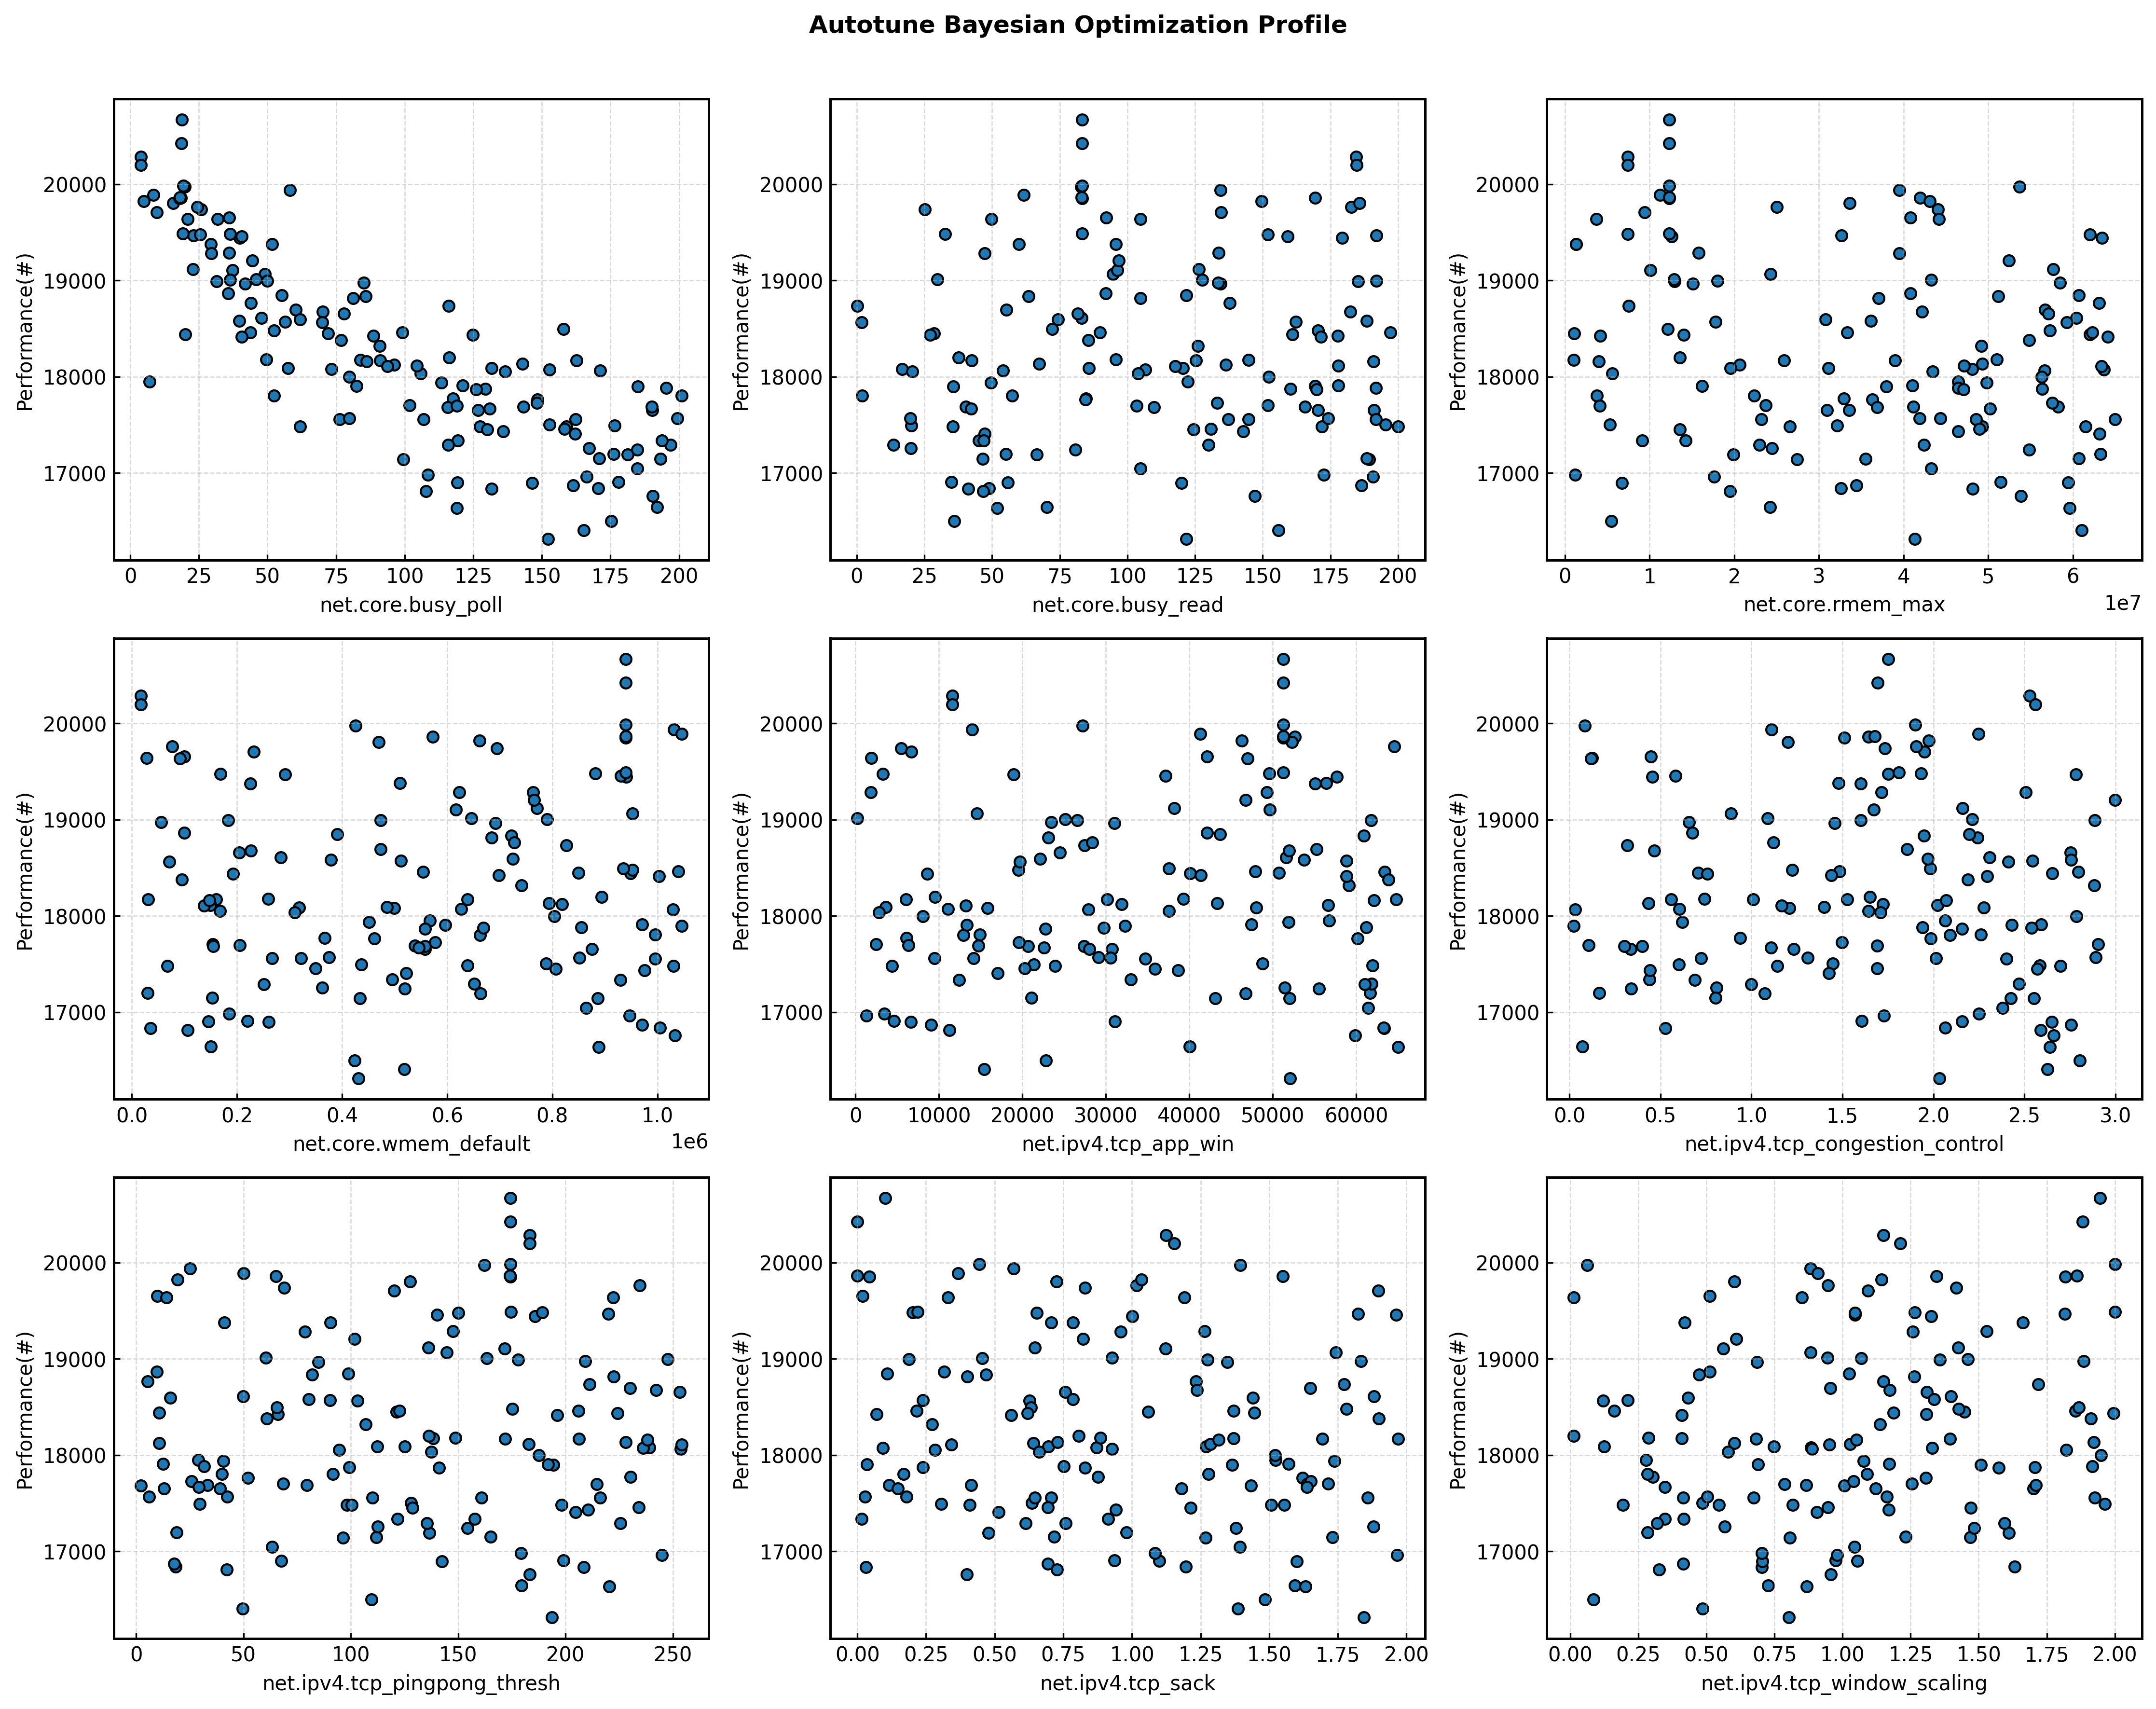
\includegraphics[width=0.85\linewidth]{images/5_evaluation/apache/profiler.png}
    \caption{Performance profile scatter plots for the Apache HTTP Server. For visual clarity, this figure displays a filtered subset of the evaluated parameters, mapping explored values against resulting application throughput. The \texttt{busy\_poll} subplot reveals a negative correlation, showing that peak throughput is exclusively achieved when the polling mechanism is effectively disabled (values clustered near zero).}
    \label{fig:apache_profiler}
\end{figure}

This requirement is conclusively proven by the top 10\% runs heat-map in Figure~\ref{fig:apache_heatmap}.
Across all best experimental runs, the optimizer aggressively clamped the normalized value of \texttt{busy\_poll} between 0.00 and 0.10, refusing to explore higher values once the penalty was mapped.
While other parameters like \texttt{tcp\_window\_scaling} and \texttt{tcp\_congestion\_control} exhibited some influence, they were entirely secondary.
For Apache, preventing thread starvation by eliminating CPU busy-polling was the absolute prerequisite for maximizing throughput.

\begin{figure}
    \centering
    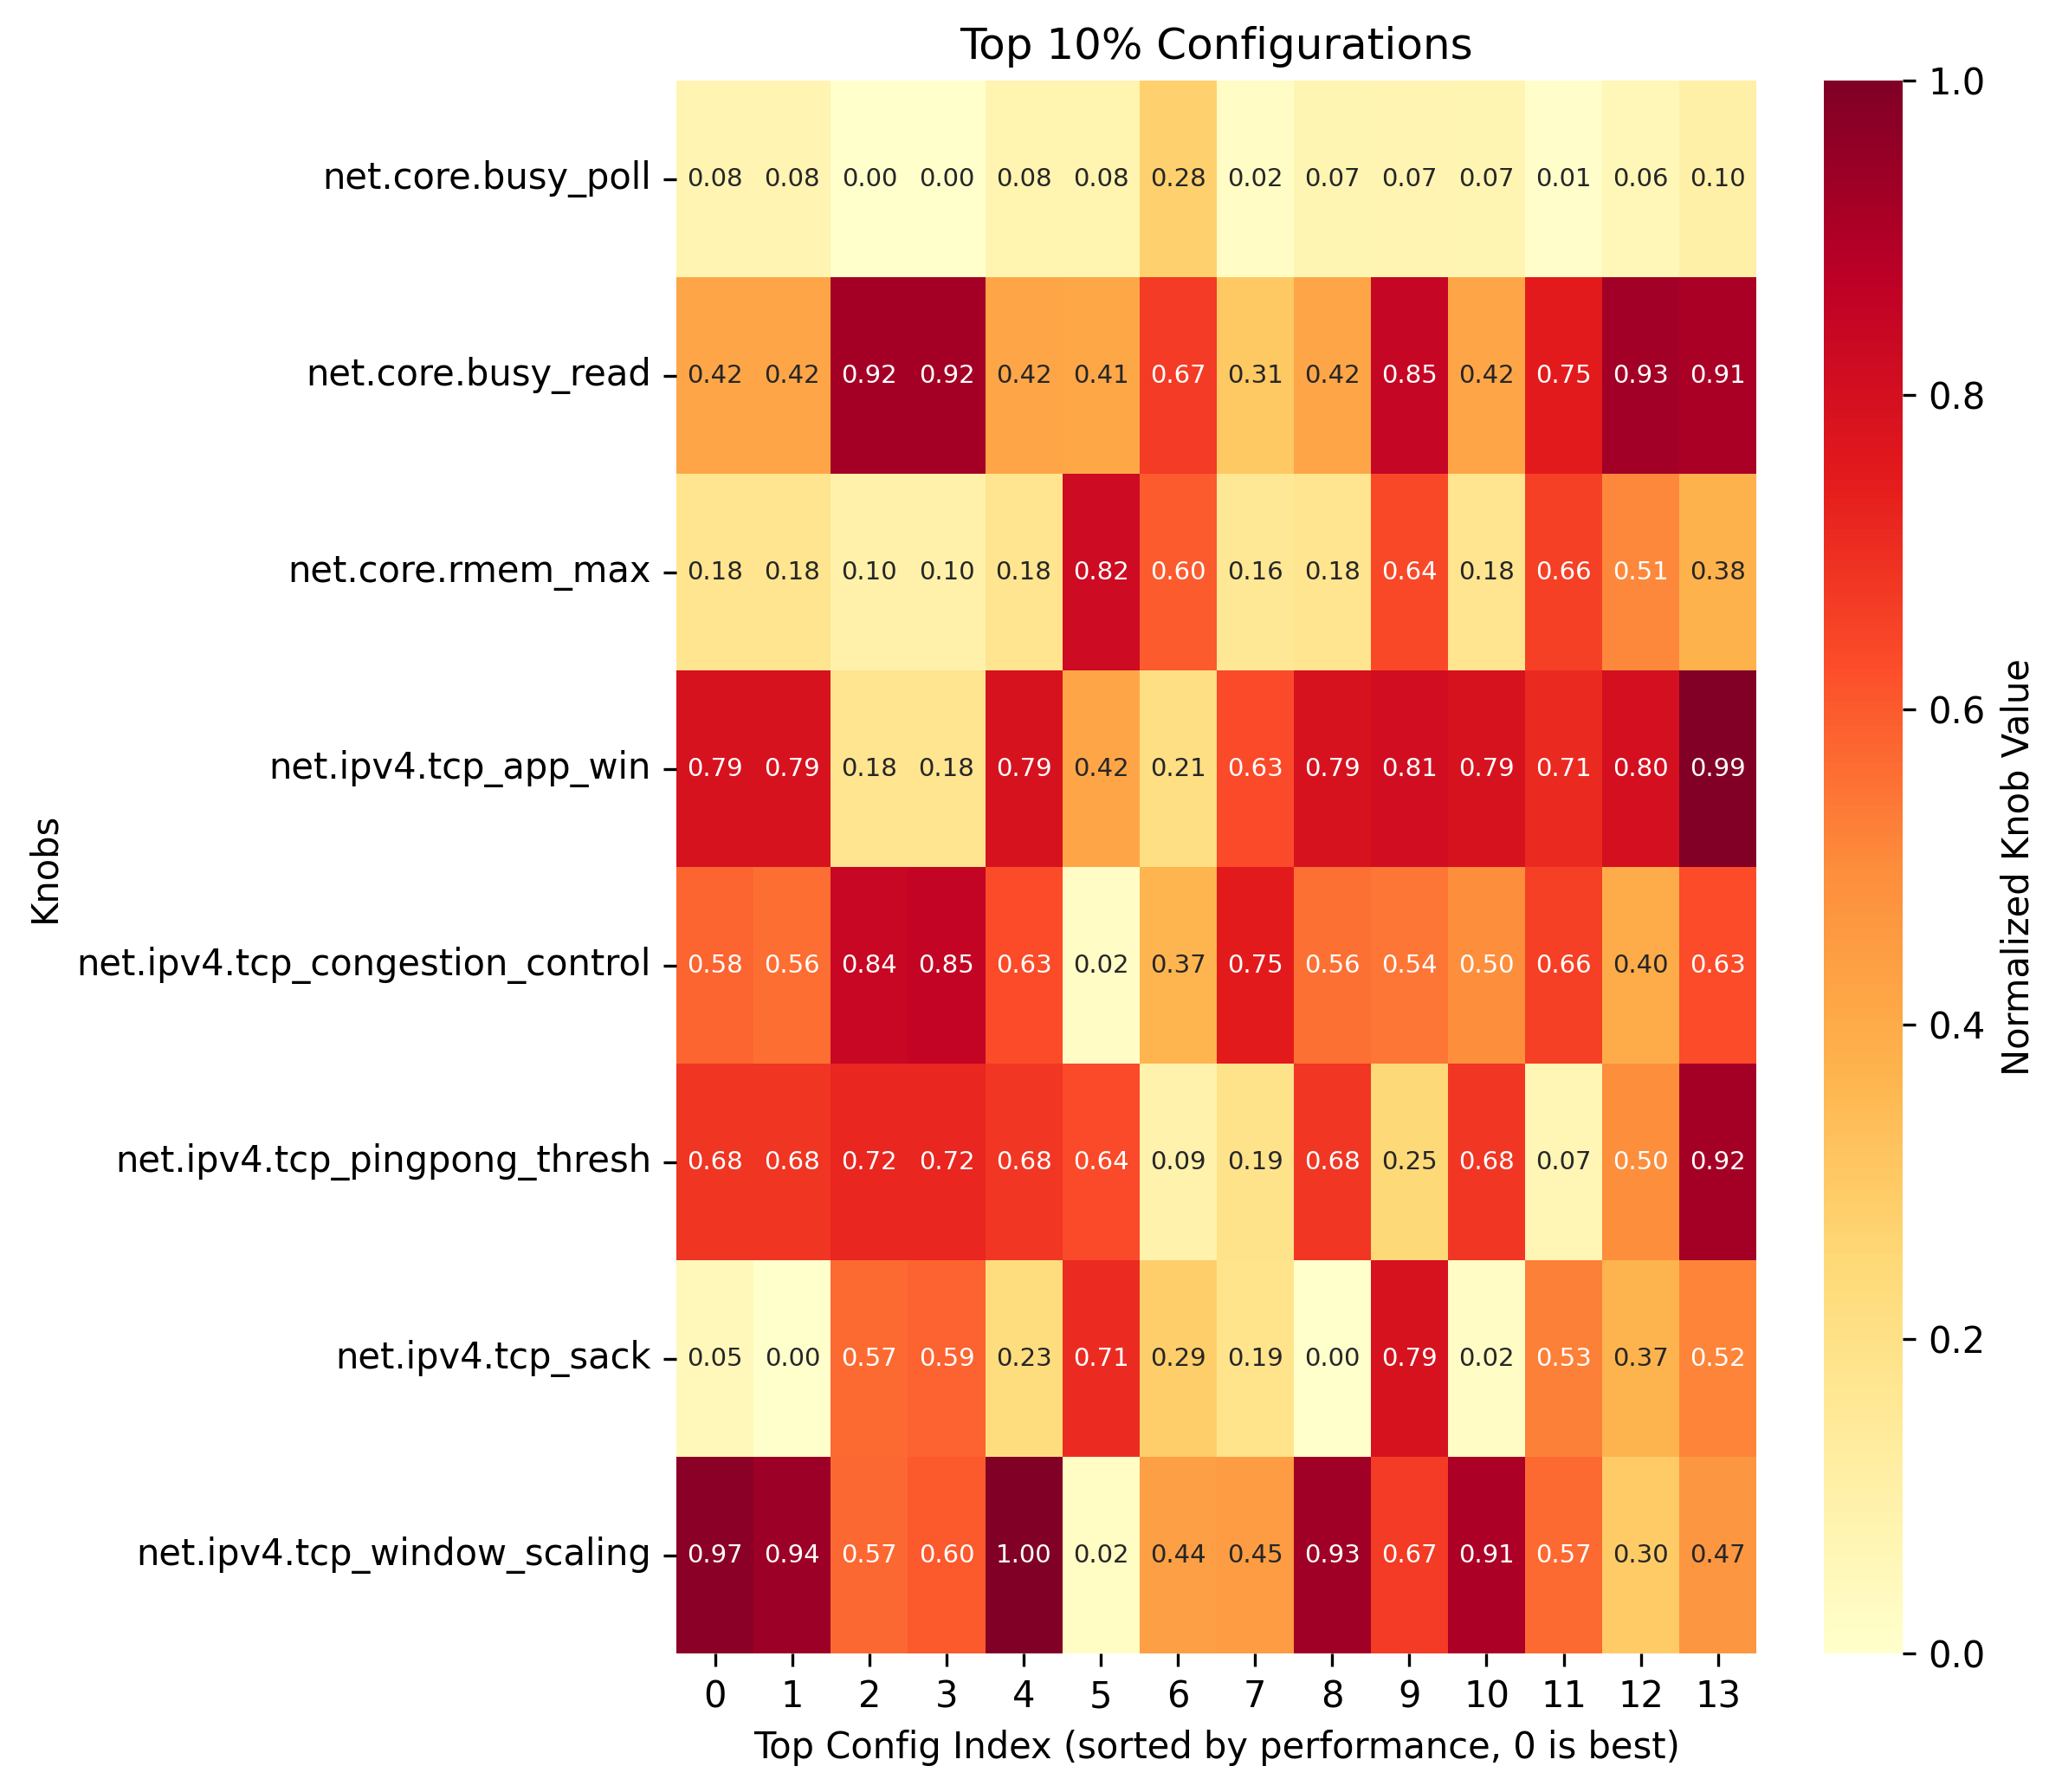
\includegraphics[width=0.7\linewidth]{images/5_evaluation/apache/heatmap.png}
    \caption{Configuration heat-map displaying the normalized parameter values across the top 10\% highest-performing experimental runs for Apache (where index 0 represents the absolute best configuration). The uniform, light-yellow shading for \texttt{busy\_poll} confirms the optimizer consistent strategy to clamp this value near 0.0 across all best configurations to prevent thread starvation.}
    \label{fig:apache_heatmap}
\end{figure}

\subsection{Workload-Specific Behaviors}

To conclusively demonstrate that optimal kernel configurations are dictated not only by the application architecture but also by its immediate traffic profile, the evaluation of NGINX was repeated using the 1KB payload workload (Workload A).
Because a 1KB file easily fits within a single network packet, this workload fundamentally alters the kernel execution path.
The system is no longer constrained by the raw data transmission mechanics (such as TCP window scaling) that dominated the 100KB tests.
Instead, the bottleneck shifts entirely to the kernel ability to rapidly establish and process thousands of transient connections per second (Figure~\ref{fig:nginx_1kb_busypoll}.

When the automated tuning framework evaluated NGINX under this high-concurrency, short-lived connection workload, the most critical parameter identified was \texttt{busy\_poll}.
However, in a stark reversal from the Apache HTTP Server results, the optimizer determined that the absolute best value for NGINX was as high as possible.
The performance profile reveals a distinct upward trend, with peak throughput achieved when \texttt{busy\_poll} is pushed toward its maximum tested limit.

This divergence perfectly highlights the interplay between workload and architecture.
Apache heavy, thread-per-connection model was severely starved of CPU cycles by busy-polling.
NGINX, however, utilizes an exceptionally lightweight, single-threaded event loop.
Because the 1KB payload requires very little user-space processing, NGINX has an abundance of CPU cycles available.
By setting \texttt{busy\_poll} to a high value, the kernel is instructed to aggressively burn those available CPU cycles by continuously polling the network device for new packets.
This bypasses the latency introduced by hardware interrupts, allowing NGINX to shave microseconds off every single request.
Over hundreds of thousands of requests, this micro-optimization compounds into a massive throughput gain.

\paragraph{Interactive TCP Dynamics.}
To uncover secondary bottlenecks, a subsequent optimization run  (Figure~\ref{fig:nginx_1kb_pingpong}) was executed with \texttt{busy\_poll} statically locked to its optimal value (200).
With the polling latency eliminated, the framework surrogate model identified \texttt{tcp\_pingpong\_thresh} as the next most critical parameter, highly favouring a value of exactly 0.

The \texttt{tcp\_pingpong\_thresh} parameter governs the kernel heuristics for identifying interactive versus bulk data connections, which directly influences the TCP delayed acknowledgment (delayed ACK) mechanism.
By default, the kernel attempts to delay ACKs to piggyback them onto outgoing data packets, which is highly efficient for continuous data streams.
However, for a 1KB workload, the interaction is purely transactional: a rapid request followed by a rapid, single-packet response.
By forcing \texttt{tcp\_pingpong\_thresh} to 0, the kernel is essentially instructed to disable delayed ACKs and treat the socket as highly interactive.
This forces immediate acknowledgments, eliminating the artificial latency introduced by waiting for the delayed ACK timer to expire, and allows the server to instantly close the connection and free the socket for the next user.

\begin{figure}[htbp]
  \centering
  
  % --- Top Row: Single Plot ---
  \begin{subfigure}{\textwidth}
    \centering
    % Restricting width to 60% so it doesn't look comically large
    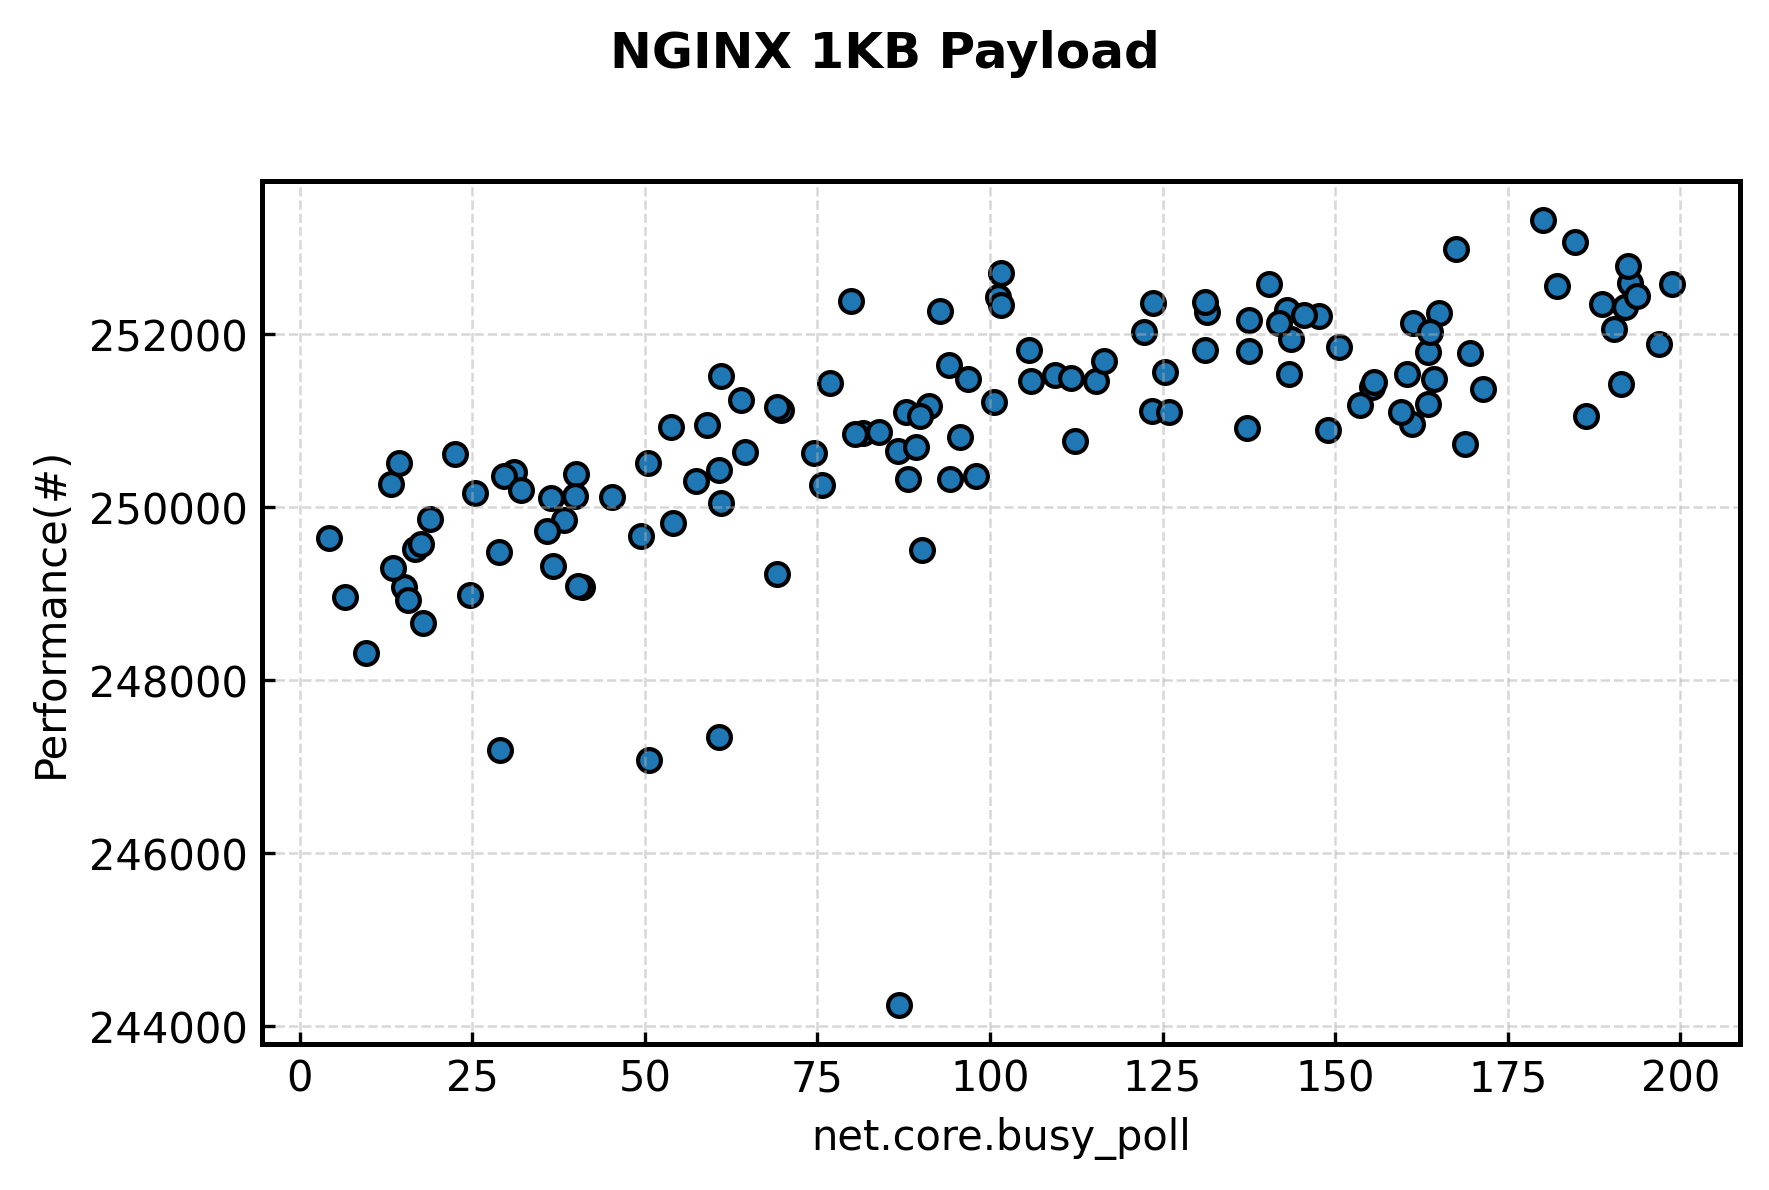
\includegraphics[width=0.6\textwidth]{images/5_evaluation/nginx/nginx_1kb_busypoll_profiler.png}
    \caption{Performance profile for NGINX under the 1KB payload workload. In contrast to thread-heavy applications, the lightweight event-driven architecture of NGINX thrives under active network polling. The scatter plot demonstrates a clear upward trajectory, achieving peak throughput when \texttt{busy\_poll} is maximized to minimize interrupt latency.}
    \label{fig:nginx_1kb_busypoll}
  \end{subfigure}
  
  \vspace{1em} % breathing room between top and bottom
  
  % --- Bottom Row: Double Plot ---
  \begin{subfigure}{\textwidth}
    \centering
    % Spanning the full text width
    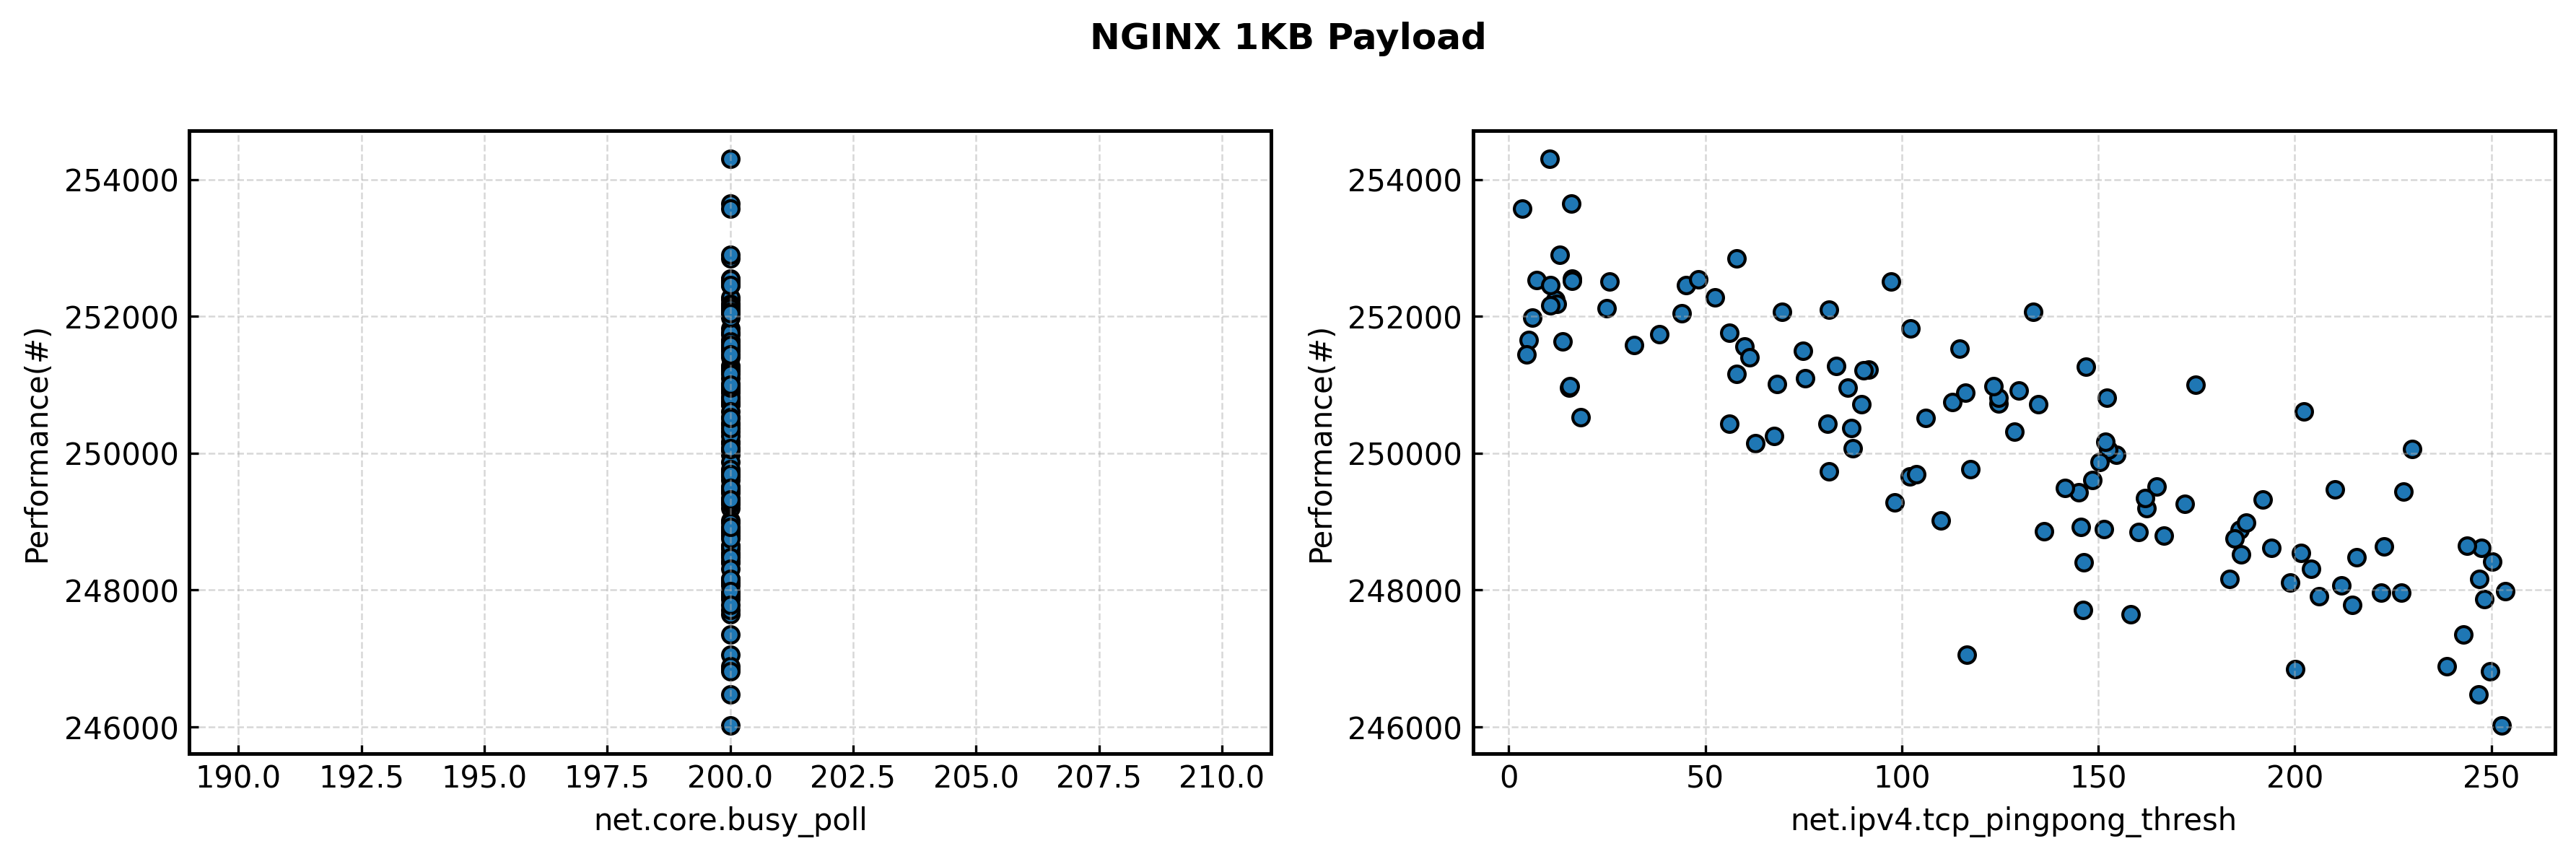
\includegraphics[width=\textwidth]    {images/5_evaluation/nginx/nginx_1kb_pingpong_profiler.png}
    \caption{Secondary performance profile for NGINX (1KB payload) generated with \texttt{busy\_poll} locked at 200. The subplot for \texttt{tcp\_pingpong\_thresh} reveals a strong negative correlation. Clamping this value to 0 disables delayed acknowledgment heuristics, forcing immediate ACKs that drastically accelerate the lifecycle of short-lived connections.}
    \label{fig:nginx_1kb_pingpong}
  \end{subfigure}
  
  \caption{Overall Autotune Bayesian Optimization Profiles for NGINX. (a) shows the isolated busy poll performance, while (b) demonstrates the ping-pong thresholds.}
  \label{fig:nginx_profiles}
\end{figure}

\section{Summary}

Ultimately, these findings confirm that a universal, "one-size-fits-all" configuration for Linux kernel parameters fundamentally does not exist.
Because optimal \textit{sysctl} values fluctuate wildly depending on user-space architectures and real-time network traffic, relying on static defaults or manual tuning is inadequate.

This underscores the core value and necessity of the methodology proposed in this thesis.
By operating entirely within the kernel space, intersecting top-down system call execution graphs with bottom-up parameter data flows, the framework successfully identifies the critical subset of tuning knobs in a strictly application-agnostic and workload-agnostic manner.
Even though the final optimal values are highly dynamic, the search space of relevant parameters is intrinsically tied to the kernel paths the application invokes.
By reducing thousands of available kernel parameters down to a targeted, execution-path-specific list, this methodology provides the essential foundation required for automated optimization tools to rapidly converge on peak system performance for any arbitrary workload.

\newpage
